\documentclass[MSc,italian]{dfaunictthesis}
\usepackage{lipsum}
\usepackage[compat=1.0.0]{tikz-feynman}
\usepackage{braket}
\usepackage{mhchem}
\usepackage{textcomp}
\usepackage{psfrag}
\usepackage{subfigure}
\usepackage{multirow}
\usepackage{booktabs}
\usepackage{ctable}
\usepackage{footnote}
%\usepackage{mathtools}
%\usepackage{mathrsfs}
%\usepackage{amsfonts}
%\usepackage{amsmath}
\usepackage{amssymb}
\usepackage{siunitx}
%\usepackage[retainorgcmds]{IEEEtrantools}
\usepackage[hypcap=true]{caption}
\usepackage[Lenny]{fncychap}
\hypersetup{
%	pdfpagemode={UseOutlines},
%	bookmarksopen,
%	colorlinks,
%	linkcolor=red,
%	anchorcolor=red,
%	citecolor=red,
%	urlcolor=red,
%	%linktocpage=true
%	pdftitle={La condensazione di Bose-Einstein},
%	pdfauthor={Giuseppe Antonio Brischetto}
}

\usepackage{url}
\usepackage{booktabs}

\newcommand{\doppiobeta}{$ 0\nu\beta\beta$}

%\newcommand{\geant}{\begin{scshape}geant4\end{scshape}}
\newcommand{\geant}{Geant4}


\begin{document}

\author{Giuseppe Antonio Brischetto}
\title{Simulazioni Monte Carlo di un sistema di rivelazione per ioni pesanti basato sulla tecnologia SiC-CsI per il progetto NUMEN}
\aayear{2018/2019}

\begin{supervisors}
   \supervisor{Chiar.mo}{Prof.}{F. Cappuzzello}
   %\supervisor{}{Dr.}{L. Pandola}
\end{supervisors}

%\phdname{physics} % default
%\phdname{science of materials}
%\phdname{complex systems}

\maketitlepage

%\tableofcontents
\thispagestyle{empty}
\cleardoublepage


\begin{flushright}
	\null \vspace{\stretch{1}}
	\textit{Ai miei genitori, Michelangelo e Concetta\\}
	\textit{A mio fratello, Alberto\\}
    \textit{Al mio amore, Carla}
    \vspace{\stretch{2}} \null
\end{flushright}

\thispagestyle{empty}
\newpage

\thispagestyle{empty}
% Le prossime righe servono per aggiungere l'indice alla barra dei segnalibri nel pdf.
\cleardoublepage
%\thispagestyle{empty}
\pdfbookmark[1]{Indice}{Indice}
\tableofcontents
%\thispagestyle{empty}
%\clearpage
%\thispagestyle{empty}

% Le prossime due righe servono per sistemare il collegamento ipertestuale nell'indice. Si è usato \cleardoublepage perché la classe è book, mentre per article si usa \clearpage. Comunque vedere ArteLateX.pdf per ogni evenienza
\cleardoublepage
\phantomsection
\addcontentsline{toc}{chapter}{\iflanguage{italian}{Introduzione}{Introduction}}
\chapter*{\iflanguage{italian}{Introduzione}{Introduction}}
\markboth{Introduzione}{Introduzione}

%A causa del suo carattere elusivo, il neutrino è una delle particelle del Modello Standard di cui si conosce meno: in primo luogo, sebbene da quando sono state osservate le sue oscillazioni di sapore è noto che possiede una massa, ma il valore esatto di tale massa è ancora sconosciuto.

%A causa del suo carattere elusivo, il neutrino è una delle particelle più misteriose del Modello Standard: in primo luogo, non conosciamo il valore esatto della sua massa, ma sappiamo soltanto dei limiti superiori. 
%Inoltre, non siamo certi nemmeno della sua natura, poiché esso potrebbe essere una particella di Dirac o una particella di Majorana.
%Inoltre, non siamo certi nemmeno della sua natura, in quanto, essendo l'unico fermione fondamentale neutro, potrebbe coincidere con la propria antiparticella, come supposto da Ettore Majorana.



Nell'ultimo decennio, l'interesse suscitato dal doppio decadimento beta senza neutrini (\doppiobeta) è cresciuto senza soluzione di continuità, come testimoniano gli innumerevoli esperimenti nati per osservarlo per la prima volta; tale fenomeno rappresenta, infatti, uno strumento fondamentale per svelare alcuni dei misteri che circondano una delle particelle più elusive dell'Universo: il neutrino. 
Il \doppiobeta{} permetterebbe non soltanto di accedere alla scala assoluta della massa del neutrino, ma anche di chiarire la sua natura fondamentale; fino ad oggi, infatti, non è noto se il neutrino è una particella di Dirac o di Majorana. 
Inoltre, dal momento che tale fenomeno viola la conservazione del numero leptonico totale, potrebbe costituire anche la prima evidenza sperimentale di fisica oltre il Modello Standard.

Per estrarre dagli esperimenti sul \doppiobeta{} le informazioni di interesse sul neutrino è necessario conoscere gli elementi di matrice nucleare (Nuclear Matrix Elements, NMEs) del processo di transizione del nucleo dallo stato iniziale a quello finale. 
%Tali NMEs sono finora noti soltanto per via teorica, presentando un quadro non privo di ambiguità.
%Tali NMEs sono finora noti soltanto per via teorica, 
%Finora, le informazioni note su tali NMEs derivano soltanto da modelli teorici, i quali presentano tra loro sostanziali discrepanze.
Tali NMEs sono finora noti soltanto per via teorica, dando luogo ad uno scenario in cui i diversi modelli mostrano tra loro sostanziali discrepanze.
Allo scopo di risolvere queste ambiguità è nato il progetto NUMEN (NUclear Matrix Elements for Neutrinoless double beta decay), il quale propone ai Laboratori Nazionali del Sud (LNS) dell'Istituto Nazionale di Fisica Nucleare (INFN) un nuovo metodo per accedere sperimentalmente ai NMEs.
Il fulcro di tale metodo è la misura di sezioni d'urto di reazioni di doppio scambio di carica (Double Charge Exchange, DCE) indotte da ioni pesanti, le quali presentano diversi aspetti in comune con il \doppiobeta.
%Questi processi sono caratterizzati da sezioni 
%Poiché il progetto intende studiare in modo sistematico tutti gli isotopi candidati al \doppiobeta{} ed essendo i processi di DCE caratterizzati da sezioni d'urto estremamente basse, è stata prevista una grande opera di ristrutturazione delle due principali infrastrutture sperimentali: il Ciclotrone Superconduttore e lo spettrometro magnetico~MAGNEX. 
Essendo i processi di DCE caratterizzati da sezioni d'urto estremamente basse (tipicamente di pochi~nb), nelle prime fasi del progetto è stato possibile analizzare soltanto alcuni dei casi rilevanti, in quanto contraddistinti da particolari condizioni favorevoli.
Tuttavia, al fine di raggiungere il suo massimo, e più ambizioso, obiettivo, il progetto intende studiare in modo sistematico tutti gli isotopi candidati al \doppiobeta{}.
Ciò rende necessario l'utilizzo di fasci di ioni con intensità molto più elevate di quelle attualmente disponibili ai LNS.
A tal fine è stata prevista una grande opera di ristrutturazione delle due principali infrastrutture sperimentali: il Ciclotrone Superconduttore e lo spettrometro magnetico~MAGNEX.
Alla fine dell'upgrade i fasci di ioni pesanti avranno un'intensità almeno due ordini di grandezza superiore a quella attuale: in quest'ottica, per il progetto è fondamentale lo sviluppo di tecnologie di frontiera, in grado di tollerare le correnti previste.
Parte integrante di NUMEN è, dunque, un'intensa attività di ricerca e sviluppo, pertinente non soltanto al campo sperimentale ma anche a quello teorico.


L'upgrade di MAGNEX prevede innanzitutto importanti cambiamenti del rivelatore di piano focale (Focal Plane Detector, FPD), che coinvolgeranno sia il sistema di tracciamento a gas sia il muro di rivelatori al silicio; in particolare, dal momento che il futuro tracciatore, a differenza di quello attuale, non potrà fornire informazioni utili all'identificazione dei prodotti di reazione, il progetto prevede la sostituzione del muro di rivelatori al silicio con uno di telescopi $\Delta E - E$ a stato solido, dedicato alla Particle IDentification (PID). 
Le esigenze di alta resistenza alle radiazioni hanno guidato verso la scelta di un primo stadio costituito da un rivelatore sottile (100~$\mu$m) al carburo di silicio (SiC), seguito da un rivelatore di stop (1~cm) allo ioduro di cesio (CsI).

%Lo scopo principale di questo lavoro di tesi consiste nel valutare se tale sistema permette di distinguere in modo efficace gli ioni nella regione di interesse per NUMEN, costituita principalmente da Ossigeno, Fluoro e Neon.
Lo scopo principale di questo lavoro di tesi consiste nello sviluppo e nell'implementazione di un tool di simulazioni per il progetto NUMEN che, per la prima volta, consenta di descrivere la cinematica di reazione, il moto degli eiettili attraverso gli elementi magnetici di MAGNEX e la loro interazione con il muro di telescopi SiC-CsI.
All'interno di tale tool, i software dedicati al calcolo della cinematica e al trasporto ottico dei prodotti di reazione sono già esistenti e ottimizzati, mentre l'applicazione che riproduce il sistema di rivelazione è stata sviluppata nel corso di questo lavoro.
Tale applicazione è stata realizzata utilizzando la piattaforma \geant{}, la quale, attraverso metodi Monte Carlo, permette di studiare l'interazione delle particelle con la materia.
Lo sviluppo di questo tool di simulazioni è estremamente importante per il progetto, in quanto coinvolge aspetti legati sia alla fase di progettazione sia alla fase operativa del sistema di rivelazione.
%In questo lavoro, il tool è stato utilizzato per analizzare le condizioni ottimali di granularità dei telescopi, valutando le capacità di PID per diverse soluzioni.
In questo lavoro, il tool è stato utilizzato per analizzare e ottimizzare le capacità di PID dei telescopi, valutando diverse soluzioni in termini di granularità.
Per ogni caso considerato si è stimata la frazione di eventi degradati, che possono costituire una minaccia dal punto di vista della PID poiché nelle matrici $\Delta E - E$ possono andare a collocarsi in regioni pertinenti ad altri ioni. 
%Lo sviluppo di questo tool permette di condurre uno studio accurato per l'ottimizzazione delle specifiche tecniche dei telescopi, quali ad esempio la granularità, 
%Grazie a questo tool di simulazioni è stato possibile condurre uno studio al fine di ottimizzare le capacità di PID del telescopio e la sensibilità di misura in diverse condizioni di granularità.
Nello studio di processi rari come quelli di DCE è, infatti, essenziale avere un'elevata sensibilità di misura delle sezioni d'urto ed un grande potere di reiezione degli eventi di fondo. 
Il lavoro svolto per questa tesi costituisce il primo passo verso lo sviluppo di una simulazione dell'intero apparato sperimentale previsto dopo l'upgrade, che riproduca fedelmente la risposta di questo agli eventi di interesse.
 
%A tal fine è stata implementata sulla piattaforma \geant{} una simulazione basata su metodi Monte Carlo, grazie alla quale è stato possibile analizzare diverse soluzioni in termini di granularità, di spessore del substrato morto e di estensione della cornice parzialmente attiva attorno alla superficie sensibile del rivelatore al SiC.
%%Per ogni caso considerato si è calcolata la frazione di eventi affetti da fenomeni di raccolta di carica incompleta, i quali possono costituire una minaccia dal punto di vista della PID poiché nelle matrici $\Delta E - E$ possono andare a collocarsi in regioni pertinenti ad altre specie atomiche.
%%Un'attenta disamina di tali eventi è cruciale al fine di garantire una bassa percentuale di errore nella PID, la quale è condizione necessaria per lo studio di processi rari come quelli di~DCE.


Nel Capitolo~1 viene illustrato il contesto scientifico che ha portato alla proposta del progetto NUMEN, descrivendo brevemente gli aspetti essenziali del \doppiobeta{} ed evidenziando le somiglianze tra questo e le reazioni di DCE.
%Vengono, inoltre, discussi gli obiettivi e le fasi del progetto, mettendo in luce l'importanza di questo lavoro di tesi nella prospettiva dell'upgrade del 
Vengono, inoltre, discusse le importanti sfide tecnologiche che il progetto si propone di affrontare al fine di raggiungere gli obiettivi fissati, mettendo in luce l'importanza di questo lavoro di tesi nella prospettiva dell'upgrade del FPD di MAGNEX.


Nel Capitolo~2 vengono presentate le principali caratteristiche dell'attuale apparato sperimentale, descrivendone in breve il principio di funzionamento.
Vengono successivamente illustrati il progetto e il principio di funzionamento del futuro FPD, dedicando particolare spazio al muro di telescopi SiC-CsI.
%Dal momento che i rivelatori al SiC rappresentano un'avanguardia nel campo dei rivelatori di particelle, ne vengono discussi gli aspetti più importanti, sottolineando le proprietà di resistenza alle radiazioni che li hanno resi adatti alle esigenze di NUMEN.
Vengono, quindi, discusse le caratteristiche più importanti dei rivelatori al SiC e degli scintillatori allo CsI, sottolineandone le proprietà di resistenza alle radiazioni, che sono state essenziali per la loro scelta nell'ambito del progetto.
Infine, viene descritto il set-up sperimentale adottato in occasione del test beam svolto ad Aprile 2019, che aveva lo scopo di valutare le performance dei primi due prototipi di telescopi SiC-CsI e del primo esemplare di elettronica di front-end per il progetto.

Nel Capitolo~3, dopo aver esposto i tratti generali delle simulazioni Monte Carlo ed averne spiegato i vantaggi nello studio di problemi ad alta complessità, viene introdotta la piattaforma \geant{}, illustrandone sinteticamente la struttura.
Vengono, dunque, descritti gli aspetti più importanti delle simulazioni svolte per questo lavoro, specificando le condizioni assunte sulla geometria, sulla generazione delle particelle primarie e sui modelli dei processi fisici.
%Infine, vengono presentati i risultati ottenuti, evidenziando nelle diverse condizioni considerate la percentuale di nuclei potenzialmente male identificati.
Infine, vengono presentati i risultati ottenuti, analizzando le performance di identificazione degli ioni al variare dei parametri rilevanti per questo studio e suggerendo le condizioni ottimali dal punto di vista della PID.
 
%Nel Capitolo~4 vengono presentati i risultati del test beam, illustrando le matrici $\Delta E - E$ ottenute.
Nel Capitolo~4 vengono presentati i risultati del test beam, illustrando le correlazioni $\Delta E - E$ ottenute nelle due configurazioni elettroniche.
Viene, dunque, descritta l'analisi svolta allo scopo di determinare dei parametri di fondamentale importanza per poter simulare le condizioni sperimentali del test.
Infine, viene mostrato il confronto tra i dati sperimentali e quelli simulati, in modo da verificarne la compatibilità.




% Queste due righe non mi sembra che servano
%\chapter*{\iflanguage{italian}{Introduzione}{Introduction}}
%\setcounter{page}{1}


%\lipsum[20]

\chapter{\iflanguage{italian}{Il contesto scientifico}{State of the art}}
Quando nel 1998 l'esperimento Super-Kamiokande ha per la prima volta osservato le oscillazioni del neutrino\cite{fukuda:prl98}, si è dimostrato inequivocabilmente che tale particella possiede una massa. 
%Tuttavia, dal momento che tale fenomeno è funzione della differenza dei quadrati delle masse, sono necessarie altre tipologie di esperimenti per accedere alla scala di massa assoluta.
Tuttavia, essendo la probabilità di oscillazione funzione della differenza dei quadrati delle masse, tale fenomeno non permette di conoscere la scala di massa assoluta. 
Altre tipologie di esperimenti sono, dunque, necessarie per accedere al valore della massa del neutrino.
Fra i processi capaci di fornire questa informazione, particolare importanza assume il doppio decadimento beta senza l'emissione di neutrini (\doppiobeta), poiché la sua osservazione permetterebbe di chiarire in modo incontrovertibile se il neutrino è una particella di Dirac o di Majorana.
Inoltre, dal momento che tale processo viola la conservazione del numero leptonico, esso costituisce uno degli esempi più rilevanti di fisica oltre il Modello Standard (MS).
Per queste ragioni il \doppiobeta{} ha attratto a sè grande interesse da parte della comunità scientifica e nell'ultimo decennio innumerevoli esperimenti sono nati in tutto il mondo per osservarlo per la prima volta.
%come testimoniano gli innumerevoli esperimenti volti a misurarne il tempo di dimezzamento. 
%
%
%Il grande interesse della comunità scientifica sul \doppiobeta{} è testimoniato dagli innumerevoli esperimenti che in tutto il mondo provano a misurarne il tempo di dimezzamento.
% OPPURE POTREI SCRIVERE
%Questo processo ha attratto grande interesse da parte della comunità scientifica, come testimoniano gli innumerevoli esperimento che in tutto il mondo provano a misurarne il tempo di dimezzamento.
%
%
%
%Come evidenziato nella Sezione~\ref{sez:progetto_numen}, nell'espressione della probabilità di decadimento del \doppiobeta{} è presente un termine legato alla transizione del nucleo atomico dallo stato iniziale a quello finale. L'accesso per via sperimentale a tale termine è l'obiettivo principale del progetto NUMEN\cite{cappuzzello:epja18} (NUclear Matrix Elements for Neutrinoless double beta decay).  
%
%Come evidenziato nel seguito di questo capitolo, noto il tempo di dimezzamento del \doppiobeta{}, la deduzione della massa del neutrino è subordinata alla conoscenza dell'elemento di matrice che esprime la transizione del nucleo atomico dallo stato iniziale a quello finale. 
%
%L'accesso per via sperimentale a tale elemento di matrice è l'obiettivo principale del progetto NUMEN\cite{cappuzzello:epja18} (NUclear Matrix Elements for Neutrinoless double beta decay).
%
Dal momento che il \doppiobeta{} prevede transizioni fra nuclei atomici, una sua completa descrizione non può prescindere dalla struttura nucleare; in particolare, come mostrato nella~\ref{eq:rate_doppio_beta}, il tempo di dimezzamento dipende dall'elemento di matrice nucleare del processo.
%che esprime la transizione del nucleo dallo stato iniziale a quello finale. 
Il progetto NUMEN\cite{cappuzzello:epja18} (NUclear Matrix Elements for Neutrinoless double beta decay) ha come obiettivo principale l'accesso per via sperimentale a tale elemento di matrice.
%, come verrà spiegato nel seguito di questo capitolo.
\vspace{1cm}
 
In questo capitolo, dopo aver presentato le principali caratteristiche del \doppiobeta{}, vengono spiegate le motivazioni che hanno portato alla nascita di NUMEN, descrivendo le ambiziose sfide scientifiche e tecnologiche che il progetto intende affrontare e sottolineando l'importanza delle simulazioni all'interno di tale scenario.


%Il presente lavoro di tesi si colloca all'interno del progetto NUMEN\cite{cappuzzello:epja18} (NUclear Matrix Elements for Neutrinoless double beta decay), il quale propone un nuovo metodo per estrarre informazioni basate sui dati sperimentali sugli elementi di matrice nucleare che entrano in gioco nell'espressione del rate di dimezzamento del doppio decadimento beta senza neutrini (\doppiobeta). 
%Il \doppiobeta{} costituisce una delle aree di interesse più importanti della fisica contemporanea, come testimoniano gli innumerevoli esperimenti che nel mondo mirano alla sua scoperta.
%Come testimoniano gli innumerevoli esperimenti che nel mondo mirano alla sua scoperta, il \doppiobeta{} costituisce una delle aree di interesse più importanti della fisica contemporanea, dal momento che diverse questioni aperte del Modello Standard potrebbero trovare risposta nel caso in cui venisse osservato.


\section{\iflanguage{italian}{Il doppio decadimento beta senza neutrini}{The neutrinoless double beta decay}} \label{sez:doppio_beta_senza_neutrini}

L'idea del doppio decadimento beta fu per la prima volta suggerita da Maria Goeppert-Mayer nel 1935 in un articolo in cui si calcolava la probabilità di emissione simultanea di due elettroni e due \textcolor{red}{anti-neutrini (nell'articolo lei dice neutrini)} come un effetto del secondo ordine della teoria di Fermi del decadimento beta\cite{goeppert-mayer:pr35}. 
%Tale processo, oggi noto come doppio decadimento beta con due neutrini ($ 2\nu\beta\beta $), è contemplato all'interno del MS come un effetto del secondo ordine del decadimento beta.
Tale processo, oggi noto come doppio decadimento beta con due neutrini ($ 2\nu\beta\beta $), è contemplato all'interno del MS ed è stato osservato in undici isotopi, diventando il più raro e lento fenomeno naturale conosciuto.
 
%Il doppio decadimento beta con due neutrini ($ 2\nu\beta\beta $) è previsto all'interno del MS come un effetto del secondo ordine


%Il \doppiobeta{} è invece un processo proibito dal MS ed è possibile soltanto se il neutrino possiede una massa e coincide con la propria antiparticella, ovvero ....
Il \doppiobeta{} fu per la prima volta proposto da Furry nel 1939\cite{furry:pr39}, a seguito di un articolo di Majorana del 1937\cite{majorana:nc37} in cui il fisico catanese formulava l'ipotesi che il neutrino coincidesse con la propria antiparticella, ovvero fosse una \emph{particella di Majorana}. 
%soltanto se il neutrino possiede una massa ed è una particella di Majorana il \doppiobeta{} può avvenire.
%Nell'articolo di Furry veniva evidenziato come il \doppiobeta{} avesse un ruolo cruciale per fare luce sulla natura del neutrino; tale fenomeno è, infatti, possibile soltanto se il neutrino possiede una massa ed è una particella di Majorana. 
Nell'articolo di Furry veniva evidenziato il ruolo cruciale del \doppiobeta{} nella chiarificazione della natura del neutrino; il fenomeno in questione è, infatti, possibile soltanto se il neutrino possiede una massa ed è una particella di Majorana. 



%Proposto per la prima volta da Furry nel 1939\cite{furry:pr39}, il \doppiobeta{} è un processo di decadimento che può avvenire in uno dei modi seguenti:
%\begin{IEEEeqnarray}{rll}
%	& (A, Z) \rightarrow (A, Z+2) + 2e^{-}  & \\
%	& (A, Z) \rightarrow (A, Z-2) + 2e^{+}  & 
%\end{IEEEeqnarray}
%In letteratura il primo tipo di decadimento viene solitamente indicato con $\beta^-\beta^-$, mentre il secondo con $\beta^+\beta^+$.
%Proposto per la prima volta da Furry nel 1939\cite{furry:pr39}, il \doppiobeta{} è un processo di decadimento in cui due neutroni (protoni) in un nucleo atomico si trasformano in due protoni (neutroni) emettendo due elettroni (positroni) e nessun anti-neutrino (neutrino).
%Esso è possibile soltanto se il neutrino ha massa e coincide con la propria antiparticella, ovvero se è una particella di Majorana.
Il \doppiobeta{} è un processo di decadimento in cui due neutroni (protoni) in un nucleo atomico si trasformano in due protoni (neutroni) emettendo due elettroni (positroni) e nessun anti-neutrino (neutrino).
%Dal momento che vengono prodotti due elettroni, la conservazione del numero leptonico viene violata di due unità, rendendo il processo proibito secondo il~MS.
La creazione di due leptoni senza la presenza della corrispondente componente antileptonica implica che la conservazione del numero leptonico venga violata di due unità, rendendo il processo proibito secondo il MS. 
Sebbene fino ad oggi tale violazione non sia mai stata osservata, le teorie che descrivono l'unificazione dell'interazione elettrodebole e quella forte (Grand Unification Theories, GUTs) sono concordi nell'affermare che, ad energie dell'ordine di $10^{15}$ GeV, il numero leptonico cessa di essere un buon numero quantico\cite{pirro:epja06}. 
Ciò significa che il \doppiobeta{} potrebbe aprire la via verso una GUT delle interazioni fondamentali e svelare l'origine dell'asimmetria materia-antimateria presente nell'Universo\cite{vergados:ijmpe16}.
%\vspace{1cm}

Il rate di dimezzamento $ \left[ T_{1/2} \right]^{-1} $ del processo può essere espresso come il prodotto di tre fattori, ovvero
\begin{equation} \label{eq:rate_doppio_beta}
	\left[ T_{1/2} \right]^{-1} \; = \; G^{0 \nu} \: \left| M^{0 \nu} \right|^2 \: \left| f ( m_i, U_{ei}, \xi_i ) \right|^2 
\end{equation}
laddove $G^{0 \nu}$ è il fattore cinematico di spazio delle fasi dei due elettroni emessi; $ f ( m_i, U_{ei}, \xi_i ) $ è un termine contenente una combinazione delle masse $m_i$ delle tre specie di neutrini, dei coefficienti di mixing $U_{ei}$ della matrice PMNS e delle fasi di Majorana $\xi_i$; $M^{0 \nu}$ rappresenta l'ampiezza di probabilità di transizione del nucleo dallo stato iniziale $\phi_i$ a quello finale $\phi_f$, ossia
\begin{equation}
	M^{0 \nu} = \bra{\phi_f} \hat{O}^{0 \nu \beta \beta} \ket{\phi_f} 
\end{equation}
in cui $\hat{O}^{0 \nu \beta \beta}$ è l'operatore che descrive il \doppiobeta{}. 
Ad oggi i numerosi esperimenti che tentano di misurare il tempo di dimezzamento del processo sono stati in grado di fornire soltanto dei limiti inferiori; i più recenti risultati affermano che, al 90\% di livello di confidenza, $T_{1/2}$ deve essere maggiore di $8.0 \cdot 10^{25}$~yr nel caso del \ce{^{76}Ge}\cite{agostini:prl18}, e di $1.1 \cdot 10^{26}$~yr nel caso del \ce{^{136}Xe}\cite{gando:prl16}. Tali valori corrispondono ad un limite superiore per la massa del neutrino compreso tra 120 -- 260~meV nel primo caso e tra 50 -- 160~meV nel secondo.




La quantità $M^{0 \nu}$, nota in letteratura come \emph{elemento di matrice nucleare} (\emph{Nuclear Matrix Element}, NME), viene attualmente valutata attraverso avanzati metodi di calcolo, come ad esempio la Quasi-particle Random Phase Approximation (QRPA), il Large-scale Shell Model, l'Interacting Boson Model (IBM), l'Energy Density Functional (EDF) e i calcoli Ab-initio (\textcolor{red}{aggiungere ref??}). I vari metodi differiscono essenzialmente per il model space adottato, proponendo schemi di troncamento diversi a seconda dei gradi di libertà considerati rilevanti. 
Sebbene accurate informazioni provenienti da esperimenti di singolo scambio di carica (Single Charge Exchange, SCE), reazioni di transfer e cattura elettronica siano state utilizzate per porre dei vincoli ai calcoli teorici, le differenze tra i modelli sono ancora piuttosto grandi, tanto da osservare in alcuni casi discrepanze di un fattore due o tre, come si può evincere dalla Figura~\ref{fig:NME}. 

\begin{figure} [!t]
	\centering
	\includegraphics[scale=0.4]{Grafici/NME.png}
	\caption{I valori dei NMEs in funzione del numero di neutroni calcolati secondo i modelli IBM-2 \cite{barea:prc13}, QRPA-T\"{u}\cite{simkovic:prc13} e ISM\cite{menendez:npa08}. Figura tratta da~\cite{barea:prc15}.} \label{fig:NME}
\end{figure}



\section{\iflanguage{italian}{Reazioni di DCE e \doppiobeta}{DCE reactions and \doppiobeta}}


%In questo scenario appare evidente la necessità di dedurre dai dati sperimentali nuove informazioni, così da imporre limiti più stringenti ai modelli.  
Da quanto appena detto appare evidente la necessità di imporre limiti più stringenti ai modelli teorici, deducendo dai dati sperimentali nuove informazioni. 
%infatti, nonostante i NMEs non siano direttamente misurabili, sotto opportune condizioni e grazie a modelli teorici appropriati è possibile desumerne il valore tramite misure sperimentali di sezioni d'urto assolute.
In questa prospettiva, le reazioni di \emph{doppio scambio di carica} (Double Charge Exchange, DCE), ovvero le reazioni in cui la carica nucleare cambia di due unità lasciando invariato il numero di massa, si configurano come un potente strumento d'indagine sul \doppiobeta; 
%A causa della bassa sezione d'urto di tali processi, al fine di identificare le reazioni di DCE è essenziale la misura gli spettri energetici con grande risoluzione e le sezioni d'urto assolute ad angoli prossimi a zero.
infatti, sebbene i due processi siano mediati da interazioni differenti, ci sono diverse importanti similarità fra loro.
In primo luogo, gli stati nucleari inziali e finali del DCE coincidono con quelli del \doppiobeta{}, in quanto in entrambi i casi avviene la trasformazione di due neutroni (protoni) in due protoni (netroni). 
Un'altra significativa somiglianza riguarda gli operatori di transizione, i quali in tutte e due i processi contengono le componenti a corto range di Fermi, Gamow-Teller e tensoriale di rango-2, con un peso relativo che nelle reazioni di DCE dipende dall'energia incidente. 
Inoltre, in entrambi i casi nel canale intermedio virtuale l'impulso lineare è molto grande, dell'ordine di 100~MeV/c\cite{barea:prl12}. Questo è un aspetto cruciale, poiché significa che sia le reazioni di DCE sia il \doppiobeta{} sondano stati ad alto impulso della funzione d'onda nucleare, mentre altri meccanismi non ne sono in grado\cite{puppe:prc11}.

Le reazioni di DCE possono essere uno strumento utile per la comprensione del \doppiobeta{} in quanto permettono di studiare un fenomeno estremamente raro attraverso un meccanismo che, essendo guidato dall'interazione forte, possiede dei tempi caratteristici molto più brevi. 
In aggiunta, il processo di DCE ha il vantaggio di poter essere studiato attraverso misure sperimentali in un laboratorio, in una condizione che consente di tenere sotto controllo alcuni dei parametri fondamentali.
Tuttavia, l'analisi delle reazioni di DCE presenta anche degli inconvenienti: in primis, tali reazioni sono caratterizzate da sezioni d'urto molto basse, tipicamente di alcune decine di nb.
Di conseguenza, per accumulare una statistica sufficiente possono essere necessari lunghi tempi di raccolta dei dati e, a seconda dell'isotopo studiato, fasci di intensità molto grande.
Inoltre, al fine di identificare le reazioni di interesse è essenziale misurare con grande risoluzione e accuratezza sia gli spettri energetici sia le sezioni d'urto assolute ad angoli prossimi a zero. 
%Inoltre, risulta necessario misurare anche gli altri canali di reazione, in modo da  identificare e quantificare i processi di transfer di nucleoni multi-step che concorrono al meccanismo diretto. Questi contributi possono essere minimizzati grazie ad una scelta opportuna del sistema proiettile-target e dell'energia incidente.
Infine, non bisogna dimenticare che eventi così rari sono sommersi da un grande background; risulta, dunque, necessario misurare anche gli altri canali di reazione, in modo da poter identificare e quantificare i processi di transfer di nucleoni multi-step che concorrono al meccanismo diretto.




\section{\iflanguage{italian}{Il progetto NUMEN}{The NUMEN project}} \label{sez:progetto_numen}

Il progetto NUMEN propone un nuovo metodo per estrarre informazioni basate sui dati sperimentali (\textcolor{red}{meglio scrivere data-driven?}) sui NMEs che entrano in gioco nel calcolo del rate di dimezzamento del \doppiobeta{}. 
%utilizzando misure accurate di sezioni d'urto di reazioni di DCE indotte da ioni pesanti. 
Per raggiungere tale scopo si intende misurare con grande accuratezza le sezioni d'urto di reazioni di DCE indotte da ioni pesanti, esplorando a diverse energie del fascio incidente \emph{tutti} gli isotopi coinvolti negli esperimenti presenti e futuri sul \doppiobeta{}.
%In particolare, è importante verificare se le sezioni d'urto misurate del DCE sono legate ai NMEs del \doppiobeta{} come una funzione lentamente variabile dell'energia del proiettile e della massa del sistema.%cioè tipo $M^{DCE} \propto f(E_p, A, M^{0 \nu})$
%In tal caso, sarebbe possibile accedere agli elementi di matrice del \doppiobeta{} tramite misure di sezioni d'urto sperimentali. Dal punto di vista teorico, è necessario descrivere accuratamente il meccanismo di reazione, che deve essere fattorizzato in una parte di reazione ed una di struttura nucleare, con quest'ultima a sua volta fattorizzata nel termine del proiettile e in quello del bersaglio.

Il principale, e più ambizioso, obiettivo di NUMEN è l'accesso ai NMEs del \doppiobeta{} attraverso un approccio sperimentale. A tal fine bisogna verificare se gli elementi di matrice del DCE sono legati ai NMEs del \doppiobeta{} come una funzione lentamente variabile dell'energia del proiettile e della massa del sistema.
Qualora questa ipotesi fosse verificata, allora sarebbe possibile dedurre i NMEs del \doppiobeta{} a partire da misure di sezioni d'urto.
% ******* Prima avevo scritto questo:
%Se i risultati sperimentali confermassero che gli elementi di matrice del DCE sono legate ai NMEs del \doppiobeta{} come una funzione lentamente variabile dell'energia del proiettile e della massa del sistema, allora sarebbe possibile dedurre questi ultimi a partire da misure di sezioni d'urto. 
Ciò richiede che il meccanismo di reazione possa essere descritto come il prodotto di un fattore dovuto alla mera reazione e di uno relativo alla struttura nucleare, con quest'ultimo a sua volta fattorizzato in un termine del proiettile e in uno del bersaglio.
%Tale approccio si è dimostrato valido nel caso delle reazioni di singolo scambio di carica (vv. articolo Taddeucci 1987). 
Dunque, lo sviluppo di una teoria microscopica coerente della reazione di DCE è parte indispensabile del progetto. 
Dal punto di vista sperimentale, la verifica della validità di questa ipotesi richiede la costruzione di una sistematica di dati, che comprenda tutti gli isotopi soggetti al \doppiobeta.
%Sebbene per alcuni casi l'attuale apparato sperimentale possa essere sufficiente, tale studio sistematico richiede l'utilizzo di fasci di intensità molto più elevate di quelle al momento disponibili.
Poiché, come accennato nella sezione precedente, la maggior parte dei processi di DCE presenta sezioni d'urto estremamente basse, tale studio sistematico richiede l'utilizzo di fasci di intensità molto più elevate di quelle al momento disponibili.
In quest'ottica rientra la grande opera di ristrutturazione delle due principali componenti sperimentali: il Ciclotrone Superconduttore (CS) K800 e lo spettrometro magnetico MAGNEX.
%, affrontando le sfide connesse alla ricerca di fenomeni tanto rari, come la bassa sezione d'urto, la grande quantità di background, la necessità di alta risoluzione e sensibilità. 

Altro importante obiettivo di NUMEN consiste nella validazione delle teorie di struttura nucleare che si occupano di calcolare i NMEs del \doppiobeta{};
% ****** Prima avevo scritto:
%; infatti, poiché gli elementi di matrice del DCE e quelli del \doppiobeta{} contengono le stesse funzioni d'onda iniziali e finali e operatori di transizione con struttura simile, la misura di sezioni d'urto assolute può sondare la bontà dei model space adottati dai diversi metodi di calcolo.
infatti, gli elementi di matrice del DCE e quelli del \doppiobeta{} contengono le stesse funzioni d'onda iniziali e finali e operatori di transizione con struttura simile. Se scegliendo un determinato modello di struttura nucleare (con i relativi troncamenti alla funzione d'onda many-body) si trova un buon accordo con i dati sperimentali sulla sezione d'urto del DCE, allora quello stesso model space deve descrivere bene le funzioni d'onda del \doppiobeta.
% Dalla tesi di Ale: "Validare con i dati sperimentali l’applicazione di certi tagli sullo spazio di modello usato nell’analisi dei dati di DCE serve a validare la scelta dello stesso spazio di modello quando l’operatore non è più quello del doppio scambio di carica ma quello del decadimento 0νββ. In questo senso risulta essenziale avere il pieno controllo sulla componente di reazione della sezione d’urto."
Quindi, una volta scelte queste ultime dal confronto con le sezioni d'urto del DCE, le stesse possono essere impiegate per i NMEs del \doppiobeta{}. 

%Infine, NUMEN potrebbe fornire informazioni sulla sensibilità necessaria per la misura del tempo di dimezzamento del \doppiobeta{} a seconda dell'isotopo utilizzato. 
%Infine, NUMEN potrebbe fornire informazioni importanti sui diversi isotopi utilizzati nella ricerca del \doppiobeta{}, perché, facendo il rapporto delle sezioni d'urto assolute misurate negli esperimenti di DCE, si ottiene una stima di quanto il processo sia probabile indipendentemente dal modello adottato. Questa procedura, che consente di ridurre la presenza di eventuali errori sistematici poiché nel rapporto i due contributi si compensano, potrebbe 
Infine, NUMEN potrebbe fornire informazioni importanti sui diversi isotopi utilizzati nella ricerca del \doppiobeta{}, perché il rapporto delle sezioni d'urto assolute misurate negli esperimenti di DCE offre una stima di quanto il processo sia probabile indipendentemente dal modello assunto. 
%Questa procedura, che consente di ridurre la presenza di eventuali errori sistematici poiché nel rapporto i due contributi si compensano, potrebbe permettere di confrontare
Questa procedura consente di ridurre la presenza di eventuali errori sistematici poiché nel rapporto i due contributi si compensano.
Tale tipologia di analisi potrebbe avere un grande impatto sui futuri esperimenti sul \doppiobeta{}, in quanto potrebbe dare indicazioni su quale isotopo può essere il miglior candidato alla scoperta del processo e sulla sensibilità necessaria per la sua osservazione. 


Gli ambiziosi obiettivi di NUMEN pongono davanti numerose sfide, che richiedono lo sviluppo e l'utilizzo di tecniche innovative sia nel campo teorico sia in quello sperimentale. 
%In particolare, dal momento che il progetto prevede lo studio di tutti gli isotopi candidati al \doppiobeta{}, è necessario utilizzare fasci di intensità molto più alta di quella attualmente disponibile. 
%In questo contesto si inquadra il previsto upgrade delle infrastrutture dei Laboratori Nazionali del Sud (LNS).
%In particolare, dal momento che per studiare tutti gli isotopi candidati al \doppiobeta{} sono necessari fasci ad alta intensità, è fondamentale lo sviluppo di rivelatori capaci di sostenere un alto rate di conteggi.
%In particolare, dal momento che verranno utilizzati fasci ad alta intensità, per il progetto è fondamentale lo sviluppo di rivelatori capaci di sostenere un alto rate di conteggi; infatti, 
%In particolare, la necessità di utilizzare fasci ad elevata intensità rende di fondamentale importanza lo sviluppo di tecnologie di frontiera nell'ambito dei rivelatori ad alto rate di conteggi.
Fra queste, a causa dell'esigenza di utilizzare fasci ad elevata intensità, sono di fondamentale importanza la ricerca e lo sviluppo (R\&D) di tecnologie di frontiera nell'ambito dei rivelatori ad alto rate di conteggi.
%In questo tipo di attività le simulazioni costituiscono un potente strumento per valutare se le performance di un sistema di rivelazione possono soddisfare ai requisiti necessari, evitando così di dedicare tempo e risorse su soluzioni inefficaci.
In questo tipo di attività le simulazioni costituiscono un potente strumento per valutare se una soluzione può soddisfare ai requisiti necessari, evitando così di dedicare tempo e risorse su proposte inefficaci.

In questo contesto si colloca il ruolo del presente lavoro di tesi, che ha contribuito all'analisi attraverso simulazioni Monte Carlo delle prestazioni di un sistema di rivelazione a stato solido per l'identificazione di ioni pesanti.
%All'interno del progetto NUMEN, il presente lavoro di tesi ha contribuito all'analisi attraverso simulazioni Monte Carlo delle prestazioni di un sistema di rivelazione a stato solido per l'identificazione di ioni pesanti.


%L'attuale sistema di rivelazione, basato su pad di silicio, verrebbe danneggiato da tali intensità, quindi servono rivelatori con robustezza alle radiazioni.
%In particolare, è previsto una profonda trasformazione delle due principali infrastrutture sperimentali dell'intero progetto: il Ciclotrone Superconduttore (CS) K800 e lo spettrometro magnetico MAGNEX. 
%Sebbene per alcuni casi 

%L'upgrade dei lns è parte integrante del progetto.

\section{\iflanguage{italian}{L'upgrade dell'apparato sperimentale}{Upgrade of the experimental set-up}}

Come anticipato nella sezione precedente, al fine di studiare in modo sistematico tutti gli isotopi candidati al \doppiobeta{} è necessario utilizzare fasci di intensità molto più alte di quelle disponibili con l'attuale infrastruttura. Dunque, parte integrante di NUMEN è l'upgrade delle due componenti chiave del progetto, il CS e MAGNEX. 
È previsto che, alla fine del processo di ristrutturazione, l'apparato sperimentale possa essere in grado di lavorare con una corrente aumentata di due o tre ordini di grandezza, passando dalle attuali $10^{12}$~pps a circa $10^{14}$~pps (\textcolor{red}{numeri giusti?}).
%Poiché l'aumento della corrente deve essere di due o tre ordini di grandezza
Questo obiettivo può essere raggiunto soltanto a seguito di importanti cambiamenti nelle tecnologie utilizzate nell'estrazione e nel trasporto del fascio, nella realizzazione dei bersagli e nel sistema di rivelazione degli eiettili (\textcolor{red}{eiettili non esiste in italiano: lo uso lo stesso?}). 
In particolare, per quanto riguarda quest'ultimo aspetto, i principali cambiamenti previsti sono:
\begin{itemize}
	\item[--] l'aumento della massima rigidità magnetica accettata;
	\item[--] la sostituzione dell'attuale tracciatore a gas, basato su una tecnologia a fili, con un sistema che utilizza i rivelatori Thick-GEM (\textcolor{red}{giusto?});
	\item[--] la sostituzione dell'attuale muro di rivelatori a pad di silicio con una matrice di rivelatori di più piccola taglia e con migliori proprietà di resistenza alle radiazioni;
	\item[--] lo sviluppo di una matrice di rivelatori attorno al bersaglio per la misurazione dei raggi gamma emessi nella diseccitazione degli stati nucleari popolati nelle reazioni di DCE.
\end{itemize}
%Dunque, la necessità di sostenere alti rate di particelle porterà ad un profondo cambiamento dell'attuale rivelatore di piano focale (Focal Plane Detector, FPD) di MAGNEX, descritto nel capitolo successivo (\textcolor{red}{aggiungere la sezione}).
Dunque, al fine di raggiungere gli obiettivi preposti da NUMEN è necessaria una profonda trasformazione dell'attuale rivelatore di piano focale (Focal Plane Detector, FPD) di MAGNEX, descritto nel capitolo successivo (\textcolor{red}{agg sezione}).


%Dei cambiamenti precedentemente elencati particolare attenzione merita quello del tracciatore a gas 
%È importante sottolineare un aspetto dei cambiamenti precedentemente elencati: la sostituzione dell'attuale tracciatore a gas con un sistema 
Dei cambiamenti precedentemente elencati è importante sottolineare un aspetto: il presente sistema di tracciamento, oltre a fornire accurate informazioni sulla posizione, è sensibile alla perdita di energia degli ioni nel gas. Esso viene, quindi, utilizzato anche come stadio $\Delta E$ per l'identificazione in numero atomico ($Z$) dei prodotti di reazione.
La tecnologia delle Thick-GEM, scelta perché promette buone proprietà di misura della posizione anche in presenza di alti rate, non è invece in grado di dare informazioni sull'energia persa dagli ioni.
Inoltre, gli attuali rivelatori a larga area al silicio, usati per misurare l'energia residua ($ E_r $), non soltanto verrebbero danneggiati da rate così alti, ma sarebbero anche soggetti ad un significativo pile-up a causa delle loro grandi dimensioni.
Di conseguenza, per non diminuire le attuali capacità complessive di identificazione delle particelle (Particle IDentification, PID) è necessario introdurre nel FPD un sistema dedicato a questo scopo.



\subsection{\iflanguage{italian}{Il nuovo sistema di identificazione delle particelle}{The new system of particle identification}}


Il requisito fondamentale che il nuovo sistema di PID deve soddisfare è l'identificazione degli ioni nella regione dell'ossigeno (O), del fluoro (F) e del neon (Ne). 
Oltre a questo, esso deve possedere le seguenti caratteristiche:
\begin{enumerate}
	\item alta resistenza alle radiazioni (\textcolor{red}{aggiungere numeri per quantificare?});
	\item la risoluzione energetica deve essere sufficientemente buona da garantire una chiara identificazione dei prodotti di reazioni di interesse per NUMEN;
	\item il grado di segmentazione deve essere scelto in modo da mantenere la probabilità di eventi con double-hit inferiore al 3\%;
	\item l'efficienza geometrica deve essere sufficientemente alta da ridurre al minimo il background costituito dagli eventi con raccolta di carica parziale;
	\item lo spessore dei rivelatori deve riuscire a fermare gli eiettili di interesse in un grande range di energia di incidenza;
	\item i rivelatori devono essere facilmente costruibili e maneggiabili e avere un costo ragionevole.
\end{enumerate}


Dopo aver valutato diverse opzioni, tra cui i phoswich, si è scelto di utilizzare un muro di telescopi $ \Delta E - E $ a stato solido.
Negli esperimenti di fisica nucleare questo tipo di sistema è tipicamente composto da uno stadio $\Delta E$ sottile al silicio, seguito da un rivelatore spesso al silicio o da uno scintillatore per fermare lo ione. (\textcolor{red}{C'è bisogno di mettere un accenno alla Bethe-Bloch?}) 
Poiché, come già detto in precedenza, i rivelatori al silicio non possiedono le proprietà di resistenza alle radiazioni necessarie per il progetto, la scelta è oggi indirizzata verso un telescopio in cui il primo stadio è costituito da un rivelatore sottile (100~$\mu $m) al carburo di silicio\cite{tudisco:sensors18} (SiC), mentre il rivelatore di stop è uno scintillatore allo ioduro di cesio (CsI) spesso 1~cm.

%Il principale scopo del presente lavoro di tesi è stato la valutazione 
Al fine di verificare se questa scelta possa garantire le performance di PID e la risoluzione energetica necessarie per gli obiettivi del progetto, è stata implementata una simulazione Monte Carlo sulla piattaforma GEANT4\cite{agostinelli:nima02}.
Tale simulazione, che costituisce l'argomento centrale del presente lavoro di tesi, ha anche lo scopo di valutare la migliore soluzione in termini di granularità, stimando il numero di eventi con raccolta di carica incompleta.








\section{\iflanguage{italian}{Le fasi del progetto}{The phases of the project}}

Il progetto NUMEN è articolato in quattro fasi, di cui verranno esposti i tratti più importanti. 

La \emph{Fase 1}, già completata, ha dimostrato, grazie all'esperimento pilota \ce{^{40}Ca}(\ce{^{18}O},\ce{^{18}Ne})\ce{^{40}Ar}, che è possibile estrarre informazioni sulle funzioni d'onda nucleari del \doppiobeta{} tramite lo studio di reazioni di DCE.

La \emph{Fase 2}, attualmente in corso, prevede lo svolgimento di una campagna sperimentale su alcuni isotopi di interesse, scelti come compromesso tra la rilevanza di tali isotopi per gli esperimenti sul \doppiobeta{} e le esigenze tecniche. I primi sistemi oggetto di studio sono stati $^{116}\mbox{Cd}\,  - \, ^{116}\mbox{Sn} $ e $^{76}\mbox{Ge}\,  - \, ^{76}\mbox{Se} $, sondati attraverso le reazioni (\ce{^{20}Ne}, \ce{^{20}O}) e (\ce{^{18}O}, \ce{^{18}Ne}) per esplorare il meccanismo di DCE in entrambe le direzioni. Prossimamente verrà effettuato un esperimento sulla reazione \ce{^{48}Ti}(\ce{^{18}O},\ce{^{18}Ne})\ce{^{48}Ca}. 
%Durante questa fase verrà anche ottimizzata la strategia di analisi dei dati.
Della Fase~2 fa parte anche l'attività di R\&D su rivelatori, materiali e tecnologie precedentemente descritta.

La \emph{Fase 3} comprende sia lo smontaggio dell'attuale apparato sperimentale sia l'assemblaggio del nuovo. In questa fase avrà luogo anche l'upgrade del CS e della linea di trasporto. La durata prevista è di 18 - 24 mesi.
%La \emph{Fase 3} è dedicata all'upgrade del CS e di MAGNEX: in questa fase 


La \emph{Fase 4} prevede una serie di campagne sperimentali che, grazie alle acquisite condizioni di alta intensità del fascio, comprenderà tutti gli isotopi di interesse per il \doppiobeta{}. 
Questa fase sarà dedicata al calcolo della sezione d'urto assoluta di DCE. Se l'analisi teorica sarà riuscita a sviluppare una descrizione microscopica delle reazioni di DCE, allora sarà possibile avere accesso ai NMEs del \doppiobeta{}, principale obiettivo di NUMEN.










\clearpage


\chapter{\iflanguage{italian}{L'apparato sperimentale}{Experimental set-up}} \label{cap:apparato_sperimentale}


%L'apparato sperimentale attualmente in uso ai LNS-INFN nell'ambito della Fase~2 del progetto NUMEN, costituito principalmente dallo spettrometro MAGNEX e dal Ciclotrone Superconduttore K800, viene brevemente illustrato nella prima parte di questo capitolo.
L'apparato sperimentale attualmente in uso ai LNS-INFN nell'ambito della Fase~2 del progetto NUMEN è costituito principalmente dallo spettrometro MAGNEX e dal CS.
Poiché la descrizione di tale apparato non costituisce l'argomento primario del presente lavoro di tesi, nella prima parte del capitolo ne vengono discusse soltanto le caratteristiche principali, rimandando alla vasta letteratura sul tema per informazioni più dettagliate (ad esempio~\cite{cavallaro:epja12, carbone:epja12, cappuzzello:epja16, cunsolo:epjst07}).

%Nella prima parte di questo capitolo vengono illustrate le principali caratteristiche dell'apparato sperimentale attualmente in uso ai LNS-INFN nell'ambito della Fase~2 del progetto NUMEN.
%Nella seconda parte viene descritta la configurazione dell'apparato adottata in occasione del test sui telescopi SiC-CsI svolto ad Aprile 2018, sottolineando le differenze rispetto a quella consueta.
(\textcolor{red}{Sistemare questa parte})Nella seconda parte \textcolor{red}{si parla} del test sui telescopi SiC-CsI svolto ad Aprile~2018, esponendone le motivazioni, descrivendo la configurazione dell'apparato adottata e sottolineandone le differenze rispetto a quella consueta.


\section{\iflanguage{italian}{Lo spettrometro magnetico MAGNEX}{MAGNEX magnetic spectrometer}}

Lo spettrometro magnetico MAGNEX è un dispositivo ottico a grande accettanza costituito da un quadrupolo per la focalizzazione sull'asse verticale, seguito da un dipolo per la dispersione sul piano orizzontale.
Grazie alle sue peculiarità,  MAGNEX riesce ad offrire, in un angolo solido molto grande e in un ampio range energetico, un'ottima risoluzione in energia, angolo e massa.
Ciò lo rende uno strumento ideale per l'analisi di eventi caratterizzati da sezioni d'urto molto basse, come è già stato dimostrato in~\cite{cappuzzello:epja16,pereira:plb12,oliveira:jpg13}.
Inoltre, esso consente di effettuare misure fino a zero gradi, comprendendo, dunque, la regione angolare di massimo interesse per lo studio del DCE.

La caratteristica che rende MAGNEX uno strumento unico è l'implementazione di una innovativa tecnica di ricostruzione delle traiettorie degli ioni, che consente di correggere le inevitabili aberrazioni originate dalla grande accettanza del dispositivo.
Dunque, a differenza di altri spettrometri magnetici, per MAGNEX è importante determinare non soltanto il punto di impatto sul piano focale ma anche la traiettoria completa. Ciò significa che è necessario misurare quattro parametri: una coppia, chiamata $(x_{foc}, y_{foc})$, individua il punto di impatto, l'altra, indicata con $(\theta_{foc}, \phi_{foc})$, si riferisce rispettivamente all'angolo orizzontale e a quello verticale.
%Nel paragrafo successivo verrà esplicato in che modo vengono misurati tali parametri.
Il modo in cui tali parametri vengono misurati sarà esplicato nel paragrafo successivo.

In Figura~\ref{fig:magnex} è mostrata una foto di MAGNEX, in cui è possibile notare, andando da sinistra verso destra, la camera di scattering, il quadrupolo, il dipolo e il~FPD (\textcolor{red}{Aggiungere le scritte sull'immagine}).

\begin{figure} [!t]
	\centering
	\includegraphics[width=\textwidth, keepaspectratio]{Grafici/magnex.jpg}
	\caption{Lo spettrometro magnetico MAGNEX.} \label{fig:magnex}
\end{figure}



%\clearpage 

\subsection{\iflanguage{italian}{Il rivelatore di piano focale}{The Focal Plane Detector}} \label{sez:fpd}

\begin{figure} [!p]
	\centering
	\includegraphics[width=\textwidth, keepaspectratio]{Grafici/fpd.png}
	\caption{Rappresentazione schematica del FPD: a) vista laterale; b) vista dall'alto. Figura tratta da~\cite{cappuzzello:epja18}.} \label{fig:fpd}
\end{figure}

L'attuale FPD di MAGNEX, la cui rappresentazione schematica è riportata in Figura~\ref{fig:fpd}, è un sistema di rivelazione ibrido, costituito da un tracciatore a gas a bassa pressione e da un muro di rivelatori al silicio.
Esso è posizionato a 1.91~m dall'uscita del dipolo e, al fine di minimizzare gli effetti dovuti alle aberrazioni cromatiche\cite{cunsolo:nima01}, è inclinato di 59.2\textdegree{} rispetto ad un piano perpendicolare all'asse ottico.
Una finestra di mylar spessa 1.5~$\mu$m è utilizzata per contenere il gas, solitamente costituito da N35 isobutano, segnando l'ingresso nel volume attivo.




%Il tracciatore a gas è formato da un sistema di sei fili al tungsteno placcati in oro, posti al di sotto di un anodo segmentato in pad. 
%Il tracciatore a gas lavora secondo il principio tipico delle camera a deriva.
%Il tracciatore a gas è essenzialmente una camera a deriva, in cui un sistema misto di fili e pad consente la misura dei quattro parametri necessari.
%Il tracciatore a gas, che consente la ricostruzione tridimensionale della traiettoria degli ioni, è formato da sei fili al tungsteno, indicati con DC\ped{\textit{i}}, e da un anodo segmentato in pad. 
%Al di sopra di ciascun filo si trova una fila di 224 pad
%Il tracciatore a gas è essenzialmente una camera a deriva, in cui un sistema costituito da sei fili (DC\ped{\textit{i}}) e da un anodo segmentato in pad consente la misura dei quattro parametri necessari per la ricostruzione tridimensionale della traccia.
%In particolare, al di sopra di ciascun filo è presente una fila di pad, le quali sono orientate parallelamente all'asse ottico.
Il tracciatore a gas, che consente la ricostruzione tridimensionale della traiettoria degli ioni, è formato da sei fili proporzionali (DC\ped{\textit{i}}) e da un anodo segmentato in sei file di pad, disposti in modo che sopra ogni filo ci sia una fila di pad.
I fili, sfruttando il principio di lavoro delle camere a deriva, danno una misura di sei posizioni verticali ($Y_i$), mentre le pad permettono di determinare sei posizioni orizzontali ($X_i$).
%Una griglia di Frisch è posta al di sotto dei fili, in quanto questi vengono anche utilizzati per misurare l'energia persa dagli ioni nel gas.
Dal momento che i fili vengono anche utilizzati per misurare l'energia persa dagli ioni nel gas, una griglia di Frisch è posta al di sotto di essi.




Il muro di rivelatori al silicio è formato da 60 pad, organizzate in 20 colonne da 3 rivelatori ciascuna. (\textcolor{red}{Aggiungo qualche dettaglio in più?})
%Ogni pad ha un'area attiva di $70 \times 50$~mm\ap{2} ed è spessa 500~$\mu$m, sufficienti per fermare i prodotti di reazioni nel range energetico di interesse. 
Essi vengono utilizzati per fermare gli ioni, misurandone l'energia residua e producendo il segnale di trigger per l'acquisizione. 

Quando una particella carica, attraversando la finestra di mylar, entra nel volume attivo, produce nel gas coppie elettrone-ione positivo, le quali, sotto l'effetto di un campo elettrico costante, migrano rispettivamente verso la griglia di Frisch e il catodo. 
%mentre gli elettroni diffondono verso la griglia di Frisch, con una velocità che per questi ultimi è di circa $3 - 5 $~cm/$\mu$s. 
%La presenza di un campo elettrico costante provoca 
%La velocità di deriva tipica degli elettroni è di $3 - 5 $~cm/$\mu$s
Dopo aver attraversato la griglia, gli elettroni giungono in prossimità dei fili DC\ped{\textit{i}}, dove, a causa dell'elevato campo elettrico, danno luogo alla moltiplicazione a valanga. 
%La carica prodotta, proporzionale all'energia persa dalla particella nel gas, induce sulle pad una distribuzione di carica, della quale si calcola il baricentro. Questa operazione avviene per le sei file di pad, in modo tale che ai sei baricentri corrispondono sei misure di posizioni orizzantali $X_i$.
Alle tensioni e pressioni utilizzate, la carica secondaria prodotta genera un segnale proporzionale all'energia persa dalla particella nel gas. 
Poiché ciò avviene per ciascuno dei sei fili, si hanno sei segnali di perdita di energia, indicati con~$\Delta E_i$.

La stessa valanga induce sulle pad una distribuzione di carica, di cui si calcola, tramite un apposito software, il centro di gravità. Anche in questo caso l'operazione si ripete per le sei file di pad, così che vengono estratte sei misure di posizioni orizzontali~$X_i$.
A questo punto, effettuando un fit lineare sulle sei posizioni~$X_i$, si ottengono $x_{foc}$ e $\theta_{foc}$ rispettivamente dall'intercetta e dal coefficiente angolare della retta.

Superata la regione del tracciatore, la particella carica arriva al muro dei rivelatori al silicio, dove si ferma producendo un segnale proporzionale alla sua energia residua~$E_{resid}$. 
Lo stesso segnale viene utilizzato per calcolare l'intervallo di tempo impiegato dagli elettroni primari prodotti nel gas per raggiungere i fili DC\ped{\textit{i}}. 
%Dal momento che tale intervallo è proporzionale allo spazio percorso, si ottengono così sei misure di posizioni verticali~$Y_i$, dalle quali, grazie ad un fit lineare, si ricavano $y_{foc}$ e $\phi_{foc}$ in maniera analoga a quanto visto per $x_{foc}$ e $\theta_{foc}$.
Dal momento che la velocità di deriva è costante, tale intervallo di tempo è direttamente proporzionale allo spazio percorso. Si ottengono, dunque, sei misure di posizioni verticali~$Y_i$, dalle quali, grazie ad un fit lineare, si ricavano $y_{foc}$ e $\phi_{foc}$ in maniera analoga a quanto visto per $x_{foc}$ e $\theta_{foc}$.

È bene ricordare che, nelle camere a deriva a fili, la maggior parte del segnale è originata dal moto degli ioni positivi e non degli elettroni.
Di conseguenza, a causa della minore velocità degli ioni, tale tipologia di rivelatori può tipicamente sostenere rate dell'ordine di pochi~kHz. 
Questo aspetto, che costituisce una delle principali limitazioni all'intensità del fascio tollerabile dall'attuale FPD, deve essere superato nell'ottica della Fase~4. 
Nasce da qui l'esigenza di sostituire l'attuale tracciatore con un sistema in grado di lavorare con un rate elevato di ioni pesanti. 


\section{\iflanguage{italian}{Il rivelatore di piano focale di NUMEN}{NUMEN Focal Plane Detector}}


%\section{\iflanguage{italian}{Il test sui telescopi SiC-CsI}{Experimental setting for the test}}
\section{\iflanguage{italian}{I telescopi SiC-CsI}{SiC-CsI telescope detectors}}

%Ad Aprile 2018 è stato svolto un test sui primi due prototipi di telescopi SiC-CsI, allo scopo di confrontarne la risposta con il sistema attualmente utilizzato.
%Ad Aprile 2018 è stato svolto un test sui primi due prototipi di telescopi SiC-CsI, allo scopo di valutarne la risposta, confrontandola con quella del sistema attualmente utilizzato.

Ad Aprile 2018 i primi due prototipi di rivelatori al SiC per il progetto NUMEN sono stati completati e resi disponibili dalla \textcolor{red}{ST-Microelectronics} (\textcolor{red}{giusto?}).
%Dopo aver realizzato 
%Per verificare se la risposta di un telescopio formato da uno stadio $\Delta E$ al SiC seguito da un cristallo di CsI poteva garantire prestazioni di identificazione degli ioni confrontabili con quelle accessibili con l'attuale apparato, è stato svolto un test per una durata complessiva di cinque giorni.
%Dal momento che tali rivelatori non sono ancora uno standard nel mondo della fisica ma rappresentano una tecnologia nuova, è stato svolto un test per verificare se le loro prestazioni possono soddisfare le esigenze di NUMEN.
Dal momento che tali rivelatori non sono ancora uno standard nel mondo della fisica ma rappresentano una tecnologia di frontiera, è stato condotto un test per analizzarne la risposta nelle condizioni sperimentali tipiche della Fase~2 di NUMEN.
%Come illustrato nel Paragrafo~\ref{sez:sistema_identif_part}, i rivelatori al SiC sono stati scelti nell'ambito del progetto per assolvere al ruolo di sistema di PID
%Sono stati, dunque, assemblati due telescopi SiC-CsI, di cui si è studiata la risposta in termini di PID.
Come illustrato nel Paragrafo~\ref{sez:sistema_identif_part}, i rivelatori al SiC sono stati scelti nell'ambito del progetto come stadio~$\Delta E$ di un telescopio SiC-CsI per l'identificazione in numero atomico dei prodotti di reazione.
%Come illustrato nel Paragrafo~\ref{sez:sistema_identif_part}, i rivelatori al SiC sono stati scelti nell'ambito del progetto per identificare i prodotti di reazione
Lo scopo principale del test era, dunque, valutare la capacità di PID di questo sistema nella regione di interesse per NUMEN, confrontandola con quella accessibile con l'attuale apparato.

%Il fascio utilizzato nel test era costituito da \ce{^{20}Ne}, mentre i bersagli erano \ce{^{197}Au} e \ce{^{12}C}
Il test è stato svolto utilizzando un fascio di~\ce{^{20}Ne} a 20~MeV/u, incidente su \ce{^{197}Au} o \ce{^{12}C}, laddove i due bersagli avevano funzioni differenti: il primo serviva per la localizzazione dello scattering elastico, il secondo per favorire la formazione dei prodotti di reazione di interesse per NUMEN, ovvero quella dell'O, del F e del Ne.






%\subsection{\iflanguage{italian}{I telescopi SiC-CsI}{SiC-CsI telescope detectors}}

\subsection{\iflanguage{italian}{I rivelatori al carburo di silicio}{Silicon carbide detectors}}


%I dispositivi al SiC costituiscono oggi una promettente realtà nel campo dei rivelatori per la fisica, 
Grazie alle sue interessanti proprietà, il SiC costituisce oggi una promettente realtà nel campo della realizzazione di rivelatori per la fisica, configurandosi come una potenziale alternativa al silicio nelle applicazioni che richiedono una grande resistenza alle radiazioni.
La larghezza della sua gap, quasi doppia rispetto a quella del silicio, se da un lato aumenta l'energia media per la produzione di una coppia elettrone-lacuna, dall'altro riduce il numero di portatori di carica generati per agitazione termica, mantenendo, dunque, un ottimo rapporto segnale-rumore. 
Recenti test\cite{tudisco:sensors18} hanno dimostrato che con un rivelatore da 100~$\mu$m di spessore è possibile ottenere una risoluzione energetica dello 0.8\%~FWHM per le particelle $\alpha$ dell'\ce{^{241}Am} a 5486~keV.


Come la maggior parte dei rivelatori a semiconduttore, i rivelatori al SiC sono costituiti da una giunzione p-n, polarizzata inversamente per aumentare l'estensione della regione svuotata e per migliorare l'efficienza di raccolta dei portatori di carica.
Quando una particella carica attraversa il rivelatore, perde energia generando coppie elettrone-lacuna, le quali, in presenza di un campo elettrico, si muovono verso gli elettrodi, producendo il segnale.



%Gli attuali limiti tecnologici alla produzione di rivelatori al SiC sono legati alla capacità di controllare le dimensioni dell'area attiva e lo spessore dei dispositivi, dal momento che essi vengono realizzati tramite crescita epitassiale su un substrato di SiC.
Gli attuali limiti tecnologici alla produzione di rivelatori al SiC sono legati alla capacità di fabbricare dispositivi con area attiva e spessori relativamente grandi, dal momento che essi vengono realizzati tramite crescita epitassiale su un substrato di SiC.
%Ciò comporta anche la presenza di una regione in cui la ... ZONA PARZIALMENTE VIVA .... NON SO BENE COME INTRODURLA
Inoltre, proprio la presenza di tale substrato può rappresentare un problema ai fini della rivelazione, in quanto costituisce uno strato morto in cui le particelle perdono energia senza che questa possa essere misurata o possono perfino fermarsi.
%Tali problematiche sono state tenute in considerazione nella simulazione svolta per questo lavoro di tesi, la quale ne ha valutato l'impatto sulle performance del previsto sistema di rivelazione. 
La simulazione svolta per questo lavoro di tesi ha tenuto in considerazione tali limiti e problematiche, valutandone l'impatto sulle performance del previsto sistema di rivelazione e suggerendo le migliori specifiche tecniche ai fini del progetto. 



\begin{figure} [!t]
	\centering
	\includegraphics[width=\textwidth, keepaspectratio]{Grafici/sic.jpg}
	\caption{I rivelatori al carburo di silicio (SiC) utilizzati nel test: a sinistra il \emph{SiC~B}, a destra il \emph{SiC~A}.} \label{fig:sic}
\end{figure}


%I due prototipi di rivelatori al SiC utilizzati nel test sono mostrati in Figura~\ref{fig:sic}; essi avevano caratteristiche differenti: uno, chiamato \emph{SiC~A}, aveva un'area attiva non segmentata di $10 \times 10$~mm\ap{2}, con uno spessore di 10~$\mu$m ed uno strato morto di 100~$\mu$m; l'altro, indicato con \emph{SiC~B}, aveva un'area attiva segmentata in quattro pad, ciascuna di $5 \times 5$~mm\ap{2}, con uno spessore di 100~$\mu$m ed un strato morto di 350~$\mu$m.

I due prototipi di rivelatori al SiC utilizzati nel test sono mostrati in Figura~\ref{fig:sic}: come è possibile notare, essi differivano innanzitutto per la segmentazione dell'area attiva, in quanto uno, chiamato \emph{SiC~A}, era costituito da un'unica pad, mentre l'altro, indicato con \emph{SiC~B}, era suddiviso in quattro regioni. 
%Inoltre, mentre il SiC~A aveva un'area attiva di $10 \times 10$~mm\ap{2}, il SiC~B presentava 
%I due telescopi SiC-CsI utilizzati nel test
Entrambi i rivelatori avevano un'area attiva complessiva di $10 \times 10$~mm\ap{2}, laddove ogni pad del SiC~B aveva un'estensione di $5 \times 5$~mm\ap{2}.
%Un'ulteriore differenza riguardava gli spessori dei due rivelatori: mentre il SiC~A era spesso 10~$\mu$m con 100~$\mu$m di strato morto, il SiC~B aveva uno spessore di 100~$\mu$m con 350~$\mu$m di .
Un'ulteriore differenza riguardava lo spessore della regione attiva dei due rivelatori: per il SiC~A era di 10~$\mu$m, mentre per il SiC~B misurava 100~$\mu$m.
Infine, entrami i rivelatori avevano uno strato morto che, mentre per il SiC~A era spesso 100~$\mu$m, per il SiC~B aveva uno spessore di~350~$\mu$m.

In occasione del test si è scelto di utilizzare soltanto due delle quattro pad del SiC~B, le quali sono state cortocircuitate tra loro in modo tale che il rivelatore avesse una superficie sensibile di $10 \times 5$~mm\ap{2}.




%I due prototipi di rivelatori al SiC utilizzati nel test presentavano caratteristiche differenti: in primo luogo avevano spessore diversi, poiché uno era spesso 10~$\mu$m, mentre l'altro 100~$\mu$m.



\subsection{\iflanguage{italian}{Gli scintillatori allo ioduro di cesio}{Caesium iodide scintillation detector}}

%\subsection{\iflanguage{italian}{I telescopi SiC-CsI}{SiC-CsI telescope detectors}}

I due rivelatori al SiC sono stati assemblati insieme ai due scintillatori allo CsI mostrati in Figura~\ref{fig:csi}. 
Questi avevano dimensioni differenti: uno (\emph{CsI~A}) era grande $1 \times 1$~cm\ap{2}, l'altro (\emph{CsI~B}) era suddiviso in quattro regioni da $1.5 \times 1.5$~cm\ap{2} ciascuna. 
%La luce di scintillazione veniva letta in entrambi i casi con un fotodiodo da $1 \times 1$~cm\ap{2}, che 
%Ognuno dei due scintillatori era accoppiato ad un fotodiodo $1 \times 1$~cm\ap{2}
A causa delle dimensioni dei rivelatori al SiC, soltanto una delle quattro aree sensibili del CsI~B è stata utilizzata.
Ciascuno dei due cristalli era accoppiato ad un fotodiodo $1 \times 1$~cm\ap{2} per la lettura della luce di scintillazione. 


\begin{figure} [!t]
	\centering
	\includegraphics[width=\textwidth, keepaspectratio]{Grafici/csi.jpg}
	\caption{I cristalli di ioduro di cesio (CsI) utilizzati nel test: a sinistra il \emph{CsI~B}, a destra il \emph{CsI~A}.} \label{fig:csi}
\end{figure}



\begin{figure} [!t]
	\centering
	\includegraphics[width=\textwidth, keepaspectratio]{Grafici/telescopi.jpg}
	\caption{I due telescopi SiC-CsI utilizzati nel test: a sinistra il \emph{Tel~A}, a destra il \emph{Tel~B}.} \label{fig:telescopi}
\end{figure}

\clearpage

\section{\iflanguage{italian}{La configurazione dell'apparato sperimentale nel test}{Experimetal apparatus setting}}

 


\chapter{\iflanguage{italian}{La simulazione}{The simulation}} \label{cap:simulazione}




Al fine di valutare se la scelta della tecnologia SiC-CsI può soddisfare le esigenze di NUMEN è stata implementata una simulazione Monte Carlo sulla piattaforma GEANT4.
In questo capitolo vengono esposte le principali assunzioni e vengono presentati i risultati.



%Le simulazioni giocano un ruolo fondamentale nella fisica.

%In fisica, come in altre scienze, le simulazioni giocano un ruolo fondamentale, in quanto permettono di studiare la risposta di sistemi complessi tenendo sotto controllo alcuni dei suoi gradi di libertà.

\section{\iflanguage{italian}{Le simulazioni computerizzate e i metodi Monte Carlo}{Computer simulations and Monte-Carlo methods}}


In fisica, come in altre scienze, le simulazioni computerizzate giocano un ruolo fondamentale, in quanto permettono di affrontare lo studio di sistemi che sarebbero difficilmente trattabili utilizzando tecniche teoriche o sperimentali~``classiche'';
spesso, infatti, tali approcci possono presentare problematicità legate alla complessità del sistema, al tempo necessario per lo sviluppo e l'analisi, ai costi per la realizzazione di prototipi.
Introdotte negli anni Trenta grazie all'apporto di prestigiosi scienziati come von Neumann, Ulam e Fermi, il loro progresso è stato parallelo a quello dei computer, arrivando oggi ad essere uno strumento imprescindibile in molti esperimenti.
Esse forniscono una diversa prospettiva con cui guardare alla realtà, diventando in alcuni casi una base teorica da cui partire per l'interpretazione dei risultati sperimentali, oppure in altre situazioni producendo dati ``sperimentali'' con cui mettere al vaglio le teorie.


Tra i diversi metodi di simulazione computerizzata, particolare importanza hanno assunto i cosiddetti \emph{metodi Monte Carlo}~\cite{metropolis:jasa49}, il cui nome fu coniato da Metropolis ispirandosi al casinò omonimo.
%Tali metodi utilizzano la generazione di sequenze di numeri \emph{pseudo-casuali} per simulare le fluttuazioni statistiche di un sistema con un numero elevato di gradi di libertà, 
%laddove i numeri pseudo-casuali sono dei numeri prodotti in modo deterministico ma con proprietà statistiche simili a quelle dei numeri casuali.
%
Il numero di problemi che al giorno d'oggi vengono studiati utilizzando questa tecnica è enorme, annoverando campi di ricerca estremamente diversi, che vanno dalla fisica nucleare alla fisica medica, dalla meccanica statistica alla sociofisica, dall'economia alla biologia.
%Darne una definizione comprensiva di tutte le aree di interesse è un compito difficile e sostanzialmente inutile.
%
% ***** QUESTO NON ERA MALE
%Sebbene darne una definizione comprensiva di tutte le aree di interesse sia un compito difficile, in generale è possibile dire che i metodi Monte Carlo utilizzano la generazione di numeri casuali per simulare le fluttuazioni statistiche di un sistema con un numero elevato di gradi di libertà accoppiati.
%
%
Sebbene darne una definizione comprensiva di tutte le aree di interesse sia un compito difficile, in generale è possibile dire che i metodi Monte Carlo sono dei metodi numerici di risoluzione di equazioni o di calcolo di integrali basati sulla generazione di numeri casuali.
%I metodi Monte Carlo utilizzano la generazione di numeri casuali per simulare le fluttuazioni statistiche di un sistema con un numero elevato di gradi di libertà.
Il generico metodo si compone principalmente di quattro fasi:
\begin{itemize}
	\item generazione di una sequenza di numeri casuali;
	\item calcolo delle variabili di input sulla base della sequenza estratta;
	\item determinazione delle variabili di output utilizzando le variabili di input calcolate;
	\item ripetizione dei punti precedenti e analisi critica dei risultati.
\end{itemize}



%Dal momento che i metodi Monte Carlo dipendono fortemente dalla produzione veloce ed efficiente di flussi di numeri casuali, si preferisce generare le sequenze di numeri via software, piuttosto che leggerli da tavole ad hoc.
%Tuttavia, poiché tali algoritmi sono, in realtà, deterministici, 
%In realtà, dal momento che, per ragioni di velocità ed efficienza, tali sequenze sono prodotte via software, i numeri sono \emph{pseudo-casuali}
%Per risolvere un problema complesso è necessaria una sequenza molto grande di numeri casuali, i quali devono essere indipendenti fra loro.
Affinché il metodo si dimostri efficace, è essenziale che la sequenza di numeri sia quanto più possibile casuale.
Dunque, proprio la casualità con cui vengono prodotti tali numeri rappresenta il punto più delicato del metodo e, forse, il suo limite più grande; infatti, per ragioni di velocità ed efficienza i numeri vengono generati via software, invece di basarsi su processi fisici realmente casuali.
%Tuttavia, dal momento che tali algoritmi sono inevitabilmente deterministici, le sequenze di numeri sono, in realtà, \emph{pseudo-casuali}, ovvero presentano delle proprietà statistiche simili a quelle dei numeri casuali. 
Tuttavia, dal momento che tali algoritmi sono inevitabilmente deterministici, ogni numero della sequenza è univocamente calcolato a partire dal suo predecessore. 
Quindi, le sequenze di numeri sono, in realtà, \emph{pseudo-casuali}, ovvero presentano delle proprietà statistiche analoghe a quelle delle sequenze di numeri casuali, ma sono prodotte in modo deterministico. 
Per questo motivo, una successione di numeri pseudo-casuali non può avere elementi infinitamente diversi, in quanto, prima o poi, cominceranno a ripetersi.

Negli ultimi trent'anni l'importanza delle simulazioni basate su metodi Monte Carlo è cresciuta senza soluzione di continuità. 
%Uno dei motivi di tale successo deriva in quanto al crescere della complessità del problema tale tecnica risulta superiore rispetto agli approcci analitici in termini di tempo necessario per la 
%Uno dei motivi di tale successo deriva dalla maggiore efficacia di queste tecniche rispetto agli approcci analitici nella risoluzione di problemi caratterizzati da alta complessità;
%ad esempio, valutando l'efficacia di un metodo in termini del tempo necessario per risolvere un problema, al crescere della complessità risulta che tale tempo cresce più lentamente per i metodi Monte Carlo in confronto ai metodi analitici.
%come illustrato in Figura~\ref{fig:monte_carlo}, il tempo necessario 
%Uno dei motivi di tale successo deriva dalla grande efficacia di queste tecniche nella risoluzione di problemi altamente complessi;
Una delle ragioni di tale successo deriva dalla grande efficacia di queste tecniche nell'affrontare lo studio di sistemi con un numero elevato di gradi di libertà accoppiati; 
ad esempio, è possibile dimostrare che, al crescere della complessità del problema, i metodi Monte Carlo richiedono meno tempo per giungere alla soluzione rispetto alle tecniche analitiche o deterministiche, come mostrato in Figura~\ref{fig:monte_carlo}.


\begin{figure} [!t]
	\centering
	\includegraphics[scale=0.7]{Grafici/monte_carlo_vs_analytic2.png}
	\caption{Confronto fra il tempo necessario per la risoluzione di un problema con un metodo analitico-deterministico e con un metodo Monte Carlo, al variare della complessità del problema.} \label{fig:monte_carlo}
\end{figure}


%Nel campo della fisica, i metodi Monte Carlo sono spesso utilizzati per 
%Un notevole impulso allo sviluppo dei metodi Monte Carlo è provenuto dalla fisica delle alte energie, in cui l'elevata complessità degli apparati di rivelazione necessitava di uno strumento per decidere le specifiche in fase di progettazione.


%Un notevole impulso allo sviluppo dei metodi Monte Carlo è provenuto dalla fisica delle alte energie, in cui la crescente necessità di simulare complessi sistemi di rivelazione spingeva per la realizzazione di software sempre più performanti e robusti.
%
% ***** PRIMA AVEVO MESSO QUESTA
%Un notevole impulso allo sviluppo dei metodi Monte Carlo è provenuto dalla fisica delle alte energie, in cui si comprese che tali metodi offrivano la possibilità di seguire la traccia delle particelle e simulare le loro interazioni con la materia.
%
Un notevole impulso allo sviluppo dei metodi Monte Carlo è provenuto dalla fisica delle alte energie, in cui si comprese che tali metodi, offrendo la possibilità di seguire la traccia delle particelle e simulare le loro interazioni con la materia, potevano essere impiegati sia per la progettazione dei rivelatori sia per lo studio della loro risposta nelle condizioni sperimentali di interesse.
In questo contesto nacque il codice \emph{GEANT}, di cui nella sezione successiva si espongono le principali caratteristiche.





\section{\iflanguage{italian}{La piattaforma \textsc{Geant4}}{\textsc{Geant4} toolkit}}

%\section{\textsc{Geant4}}

La piattaforma GEANT, il cui nome deriva da \emph{GEometry ANd Tracking}, fu sviluppata nel 1974 al CERN di Ginevra allo scopo di simulare l'interazione di particelle elementari ad alta energia con i rivelatori.
%Questa prima versione consentiva di simulare il trasporto di un numero ristretto di particelle 
%In questa prima versione era possibile simulare soltanto un numero ristretto di particelle
In questa prima versione era possibile considerare soltanto un numero ristretto di particelle e forme geometriche semplici. 
Nel 1982 venne distribuito GEANT3, scritto in FORTRAN e nettamente potenziato rispetto al suo predecessore; infatti, si potevano simulare apparati sperimentali grandi e sofisticati e fasci di particelle molto intensi ed energetici.
Tuttavia, il codice presentava una struttura molto complessa, che rendeva difficile l'introduzione di nuove caratteristiche o la ricerca di errori.
%the simulation software geant4, which means \emph{geometry and tracking}, is a toolkit based on
%Fu così che si arrivò al 1998, anno dell'uscita dell'ultima versione del codice, chiamata \geant, interamente basata sul linguaggio C++.
%La crescente necessità di simulare complessi sistemi di rivelazione spingeva per la realizzazione di software sempre più performanti e robusti.
%
%%Fu così che nel 1998, grazie alla collaborazione di oltre 40 istituti internazionali, venne pubblicata l'ultima versione del codice, chiamata \geant.
D'altro canto, la crescente necessità di simulare complessi sistemi di rivelazione spingeva per la realizzazione di software sempre più performanti e robusti.
Fu così che nel 1998, grazie alla collaborazione di oltre 40~istituti internazionali, venne pubblicata l'ultima versione del codice, chiamata \geant.
Essa è interamente basata sul linguaggio C++, traendo vantaggio, dunque, da tutte le potenzialità offerte da una tecnologia orientata agli oggetti, come ad esempio la modularità e la compattezza.
% oppure il polimorfismo
%Il modo più corretto di definire \geant{} è \emph{toolkit}, ovvero ``cassetta per gli attrezzi'', in quanto comprende un insieme di librerie software che l'utente può selezionare a seconda delle proprie esigenze per creare un'applicazione specifica.

Oggi \geant{} consente di simulare l'interazione con la materia di tutte le particelle note, in un range energetico che va da pochi~eV fino ai~TeV.
%
%La sua notevole duttilità lo ha reso uno strumento 
Grazie alla sua notevole duttilità, sono innumerevoli gli esperimenti che si avvalgono di questo strumento e la sua area d'applicazione va dalla fisica delle alte energie, agli studi nucleari, alle applicazioni in campo medico, all'astrofisica.
Il codice è, inoltre, open-source e viene periodicamente aggiornato dalla collaborazione. 
Dal momento che la documentazione su \geant{} è ampia e dettagliata\footnote{Si veda, ad esempio, \url{www.geant4.cern.ch}}, nel prosieguo vengono presentati soltanto gli aspetti utili alla comprensione della simulazione svolta per questo lavoro di tesi.  



\subsection{\iflanguage{italian}{La struttura di \textsc{Geant4}}{\textsc{Geant4} structure}}

%Il modo più corretto di definire \geant{} è \emph{toolkit}, ovvero ``cassetta per gli attrezzi'', in quanto comprende un insieme di librerie software che l'utente può selezionare a seconda delle proprie esigenze per creare un'applicazione specifica.
Il modo più corretto di definire \geant{} è \emph{toolkit}, ovvero ``cassetta per gli attrezzi'', in quanto è costituito da un insieme di librerie software che, a seconda delle esigenze, possono essere selezionate per creare un'applicazione specifica.
L'utente deve, quindi, scrivere la sua applicazione, definendo tutti i parametri rilevanti: alcuni devono essere inseriti in modo obbligatorio, altri possono essere aggiunti facoltativamente.
%\geant{} offre numerose funzionalità:

%Ogni simulazione si compone dei seguenti aspetti: 
Nella progettazione e nella realizzazione del software, tutti gli aspetti fondamentali di un processo di simulazione sono stati inclusi:
\begin{itemize}
	\item la geometria del sistema, specificando forma, dimensione e posizione dei vari oggetti;
	\item i materiali utilizzati;
	\item la sorgente delle particelle, di cui si definisce la posizione, l'energia, la distribuzione angolare e tutte le altre caratteristiche rilevanti;
	\item i processi fisici di interazione per la modellizzazione  del comportamento delle particelle;
	%\item il tracciamento delle particelle, che può essere calcolato anche passo dopo passo, consentendo di estrarre ad ogni step informazioni legate alla particella, come ad esempio energia e posizione;
	\item il tracciamento delle particelle attraverso materiali ed, eventualmente, campi elettromagnetici esterni;
	%\item la sensitività di un rivelatore e la sua risposta;
	\item la definizione di elementi sensibili, che simulano la risposta del rivelatore;
	\item la visualizzazione tridimensionale degli oggetti simulati e delle tracce delle particelle;
	\item la generazione di dati, i quali possono essere memorizzati per una successiva analisi.
\end{itemize}


%Ciascuno degli aspetti elencati corrisponde ad una determinata \emph{classe} o \emph{categoria}, che, agendo in modo indipendente l'una dall'altra, danno al software una struttura modulare.

Gli aspetti elencati corrispondono in \geant{} a determinate \emph{classi} o \emph{categorie}, che, agendo in modo indipendente l'una dall'altra, danno al software una struttura modulare.
%Esse sono state concepite per essere facilmente estendibili o modificabili dall'utente, seguendo la logica tipica dei linguaggi orientati agli oggetti;
Esse sono state concepite per essere facilmente estendibili o modificabili, seguendo la logica tipica dei linguaggi orientati agli oggetti; infatti, grazie alla proprietà del \emph{polimorfismo}, l'utente può fornire un'implementazione alternativa delle funzioni presenti in una categoria (\textcolor{red}{provo a spiegarlo meglio introducendo le classi di base e le classi derivate?}).
%Di tutte le classi messe a disposizione, \geant{} richiede obbligatoriamente l'implementazione e l'istanziazione di tre, ovvero 
%\geant mette a disposizione un grande numero di classi, le quali sono state  concepite per essere facilmente estendibili o modificabili dall'utente, seguendo la logica tipica dei linguaggi orientati agli oggetti.
%L'implementazione e l'istanziazione di queste classi sono obbligatorie in tre casi, ovvero
%\geant{} mette a disposizione un grande numero di classi, ma per tre di loro l'implementazione e l'istanziazione sono obbligatorie.
\geant{} mette a disposizione un grande numero di classi, richiedendo obbligatoriamente l'implementazione e l'istanziazione per tre di loro: 
\begin{itemize}
	\item la classe dedicata alla definizione della geometria e dei materiali;
	\item la classe prevista per la definizione delle particelle, dei processi fisici e dei parametri di cut-off;
	\item la classe rivolta alla generazione delle particelle primarie.
\end{itemize}

Le altre classi sono, invece, opzionali e, a seconda delle esigenze, l'utente può modificarne il comportamento di default definendo la propria implementazione; ad esempio, ai fini di questo lavoro è stato necessario personalizzare la classe che rappresenta ogni ``passo'' della traccia della particella, facendo in modo che ad ogni step venisse estratta l'informazione sulla perdita di energia e sulla posizione.




\section{\iflanguage{italian}{Gli aspetti principali della simulazione}{Simulation main aspects}}

%La simulazione implementata per questo lavoro di tesi considera una matrice di telescopi SiC-CsI.
%Allo scopo di valutare le prestazioni di PID
Nell'ambito del presente lavoro di tesi è stata realizzata un'applicazione in \geant{} per simulare la risposta di un sistema di telescopi SiC-CsI agli ioni di interesse per il progetto NUMEN.
Nel seguito di questa sezione vengono illustrate nel dettaglio le caratteristiche di tale simulazione.




\subsection{\iflanguage{italian}{La geometria e i materiali}{Geometry and materials}}

Considerando un sistema di riferimento in cui l'asse $z$ è individuato dalla direzione di propagazione delle particelle, i telescopi sono fra loro separati di 2~mm lungo la direzione $x$ e di 1~mm lungo la direzione $y$.

%Ciascun telescopio è formato da tre parti: il volume attivo del rivelatore al SiC, il substrato morto dello stesso rivelatore e il cristallo allo CsI.
Ciascun telescopio è formato da due componenti, il rivelatore al SiC e il cristallo allo CsI, le quali sono poste a contatto.
Per tenere in considerazione il substrato morto del rivelatore al SiC, tale componente è, a sua volta, costituita da due parti: il volume attivo e il substrato morto.
%In accordo con le 
%
%Un importante aspetto della simulazione riguarda lo spessore dei rivelatori.


%Dal momento che nuovi sviluppi tecnologici hanno reso possibile la rimozione quasi totale del substrato, sono state svolte anche delle simulazioni in cui il suo spessore era ridotto a 10~$\mu$m. 
%Per quanto riguarda il cristallo di CsI, lo spessore è stato posto uguale a 1~cm.


%Poiché uno degli obiettivi di questo lavoro consisteva nella ricerca delle migliori condizioni di granularità,  sono stati considerati diversi valori per le dimensioni trasversali; in particolare, sulla base degli attuali limiti imposti dal processo di produzione dei rivelatori al SiC, sono state simulate aree sensibili di $1 \times 1$, $1.5 \times 1.5$ e $2 \times 2$~cm\ap{2}.
%Poiché uno degli obiettivi di questo lavoro consisteva nella ricerca delle migliori condizioni di granularità,  per le dimensioni trasversali dei telescopi sono stati presi in esame diversi valori; in particolare, sulla base degli attuali limiti imposti dal processo di produzione dei rivelatori al SiC, sono state simulate aree sensibili di $1 \times 1$, $1.5 \times 1.5$ e $2 \times 2$~cm\ap{2}.
Poiché uno degli obiettivi di questo lavoro consisteva nella ricerca delle migliori condizioni di granularità, sono state condotte diverse simulazioni al variare delle dimensioni trasversali dei telescopi; in particolare, sulla base degli attuali limiti imposti dal processo di produzione dei rivelatori al SiC, sono state simulate aree sensibili di $1 \times 1$, $1.5 \times 1.5$ e $2 \times 2$~cm\ap{2}.




%Lo spessore del primo è di 100~$\mu$m, mentre quello del secondo è di 350~$\mu$m.
%Un altro aspetto importante della simulazione riguarda lo spessore del rivelatore al SiC; infatti, sebbene la collaborazione abbia suggerito 
%Per quanto riguarda lo spessore dei due stadi del telescopio, la collaborazione aveva individuato come probabile soluzione l'utilizzo di rivelatori al SiC da 100~$\mu$m e di cristalli allo CsI di 1~cm. 

%Lo standard tecnologico attuale prevede che un rivelatore al SiC di tale spessore abbia un substrato morto spesso 350~$\mu$m.
Per quanto riguarda lo spessore dei due stadi del telescopio, in accordo con la soluzione individuata dalla collaborazione, sono stati simulati rivelatori al~SiC da 100~$\mu$m e cristalli allo CsI da 1~cm, mentre per il substrato morto si è considerato un valore di 350~$\mu$m.
%Gli spessori tenuti in considerazione erano di 100~$\mu$m per il rivelatore al SiC, di 350~$\mu$m per il substrato morto e di 1~cm per il cristallo allo CsI.
Tuttavia, dal momento che nuovi sviluppi tecnologici hanno reso possibile la rimozione quasi totale degli strati morti, si è esaminato anche il caso in cui lo spessore del substrato era ridotto a 10~$\mu$m. 
È stato, dunque, effettuato un confronto tra le due diverse condizioni, allo scopo di valutare le conseguenze sulle capacità di~PID.





%Sebbene il muro di telescopi comprenderà oltre 1000 
%La simulazione ha considerato un unico modulo di $2 \times 5$ rivelatore.
Dal momento che per gli scopi di questo lavoro non era necessario includere l'intero muro di oltre 1000 telescopi, tutte le simulazioni svolte hanno preso in esame una matrice $3 \times 3$ di elementi.
In Figura~ è mostrato l'aspetto assunto da tale matrice nella simulazione \geant.
%In Figura~ è possibile vedere la realizzazione grafica di \geant{} di un modulo $2 \times 5$ del sistema di rivelazione.




\subsection{\iflanguage{italian}{Generazione delle particelle primarie}{Primary particles generation}}

Le particelle primarie simulate comprendono tre degli ioni di maggiore interesse per NUMEN, ovvero \ce{^{18}O}, \ce{^{18}F} e \ce{^{18}Ne}. 
In alcune simulazioni sono stati coinvolti anche altri isotopi di tali specie nucleari, 








\subsection{\iflanguage{italian}{I processi fisici}{Physics process}}




\subsection{\iflanguage{italian}{Elaborazione post simulazione}{Post-simulation processing}}

\clearpage


\section{\iflanguage{italian}{I risultati}{Results}}




\chapter{\iflanguage{italian}{Validazione della simulazione \geant}{Validation of \geant simulation}}

All'interno dell'intensa campagna di studi condotta per verificare se le soluzioni previste per il progetto NUMEN possano garantire le prestazioni richieste, è stato svolto ad Aprile 2019 un test beam sui primi due prototipi di telescopi basati sulla tecnologia SiC-CsI.
Tale test si è tenuto ai Laboratori Nazionali del Sud (LNS) utilizzando un fascio di particelle di \ce{^{20}Ne} a 20~AMeV, prodotto dal Ciclotrone Superconduttore K800.
Al fine di favorire la generazione degli ioni di interesse per NUMEN, ovvero Ossigeno, Fluoro e Neon, si è scelto di utilizzare un bersaglio di \ce{^{12}C} da 400~$\mu$g/cm\ap{2}.


In questo capitolo vengono presentati i risultati ottenuti durante tale test e viene mostrato il confronto tra questi e i dati prodotti attraverso le simulazioni implementate per il presente lavoro di tesi. 
Dal momento che i prototipi utilizzati nel test presentano alcune differenze rispetto ai telescopi che verranno impiegati per NUMEN, è stato necessario modificare alcuni parametri della simulazione: in primo luogo, ricordando che, in uno dei due dispositivi (Tel~A), il primo stadio era montato in configurazione reverse, il substrato epitassiale del rivelatore al SiC è stato posto davanti al volume sensibile.
Inoltre, le dimensioni trasversali e gli spessori delle diverse componenti sono state cambiate in modo da riprodurre le caratteristiche descritte nel Paragrafo~\ref{par:telescopi}.


\section{\iflanguage{italian}{I dati del telescopio SiC-CsI}{Data of SiC-CsI telescope}}


Gli eiettili prodotti nell'interazione fra proiettile e bersaglio, dopo aver attraversato il quadrupolo e il dipolo, giungono al rivelatore di piano focale (Focal Plane Detector, FPD) di MAGNEX, dove, in occasione del test, erano stati posti i due telescopi, chiamati Tel~A e Tel~B. 
Come descritto nella Sezione~\ref{sez:test}, insieme ai due telescopi, erano stati montati quattro dei rivelatori al silicio attualmente in uso, i quali servivano da riferimento e da confronto per la Particle IDentification (PID).

Poiché all'energia utilizzata nel test i prodotti di reazione non erano in grado di superare il substrato epitassiale del Tel~B, da tale telescopio era possibile estrarre soltanto il segnale sulla perdita di energia, non permettendo di riprodurre le correlazioni $\Delta E - E_{resid}$ utili per l'identificazione in numero atomico $Z$ degli ioni.
Di conseguenza, dal momento che questo lavoro aveva lo scopo di studiare le performance di PID di tale sistema, sono stati analizzati soltanto i dati relativi al Tel~A.


%\subsection{\iflanguage{italian}{Le matrici $\Delta E_{SiC} - E_{CsI}$}{$\Delta E_{SiC} - E_{CsI}$ matrices}}

In Figura~\ref{fig:sic_csi_standard} è riportata la matrice $\Delta E_{SiC} - E_{CsI}$ registrata dal Tel~A utilizzando l'elettronica standard: come si può notare i luoghi dei diversi ioni appaiono ben separati in una regione che va dal Boro (B) al Neon (Ne).
Si può, inoltre, osservare che, poiché ai fini della PID non è necessario utilizzare la correlazione $\Delta E_{SiC} - E_{tot}$, i rivelatori non sono stati calibrati e, conseguentemente, le variabili $\Delta E_{SiC}$ e $E_{CsI}$ sono misurate in canali.


\begin{figure} [!p]
	\centering
	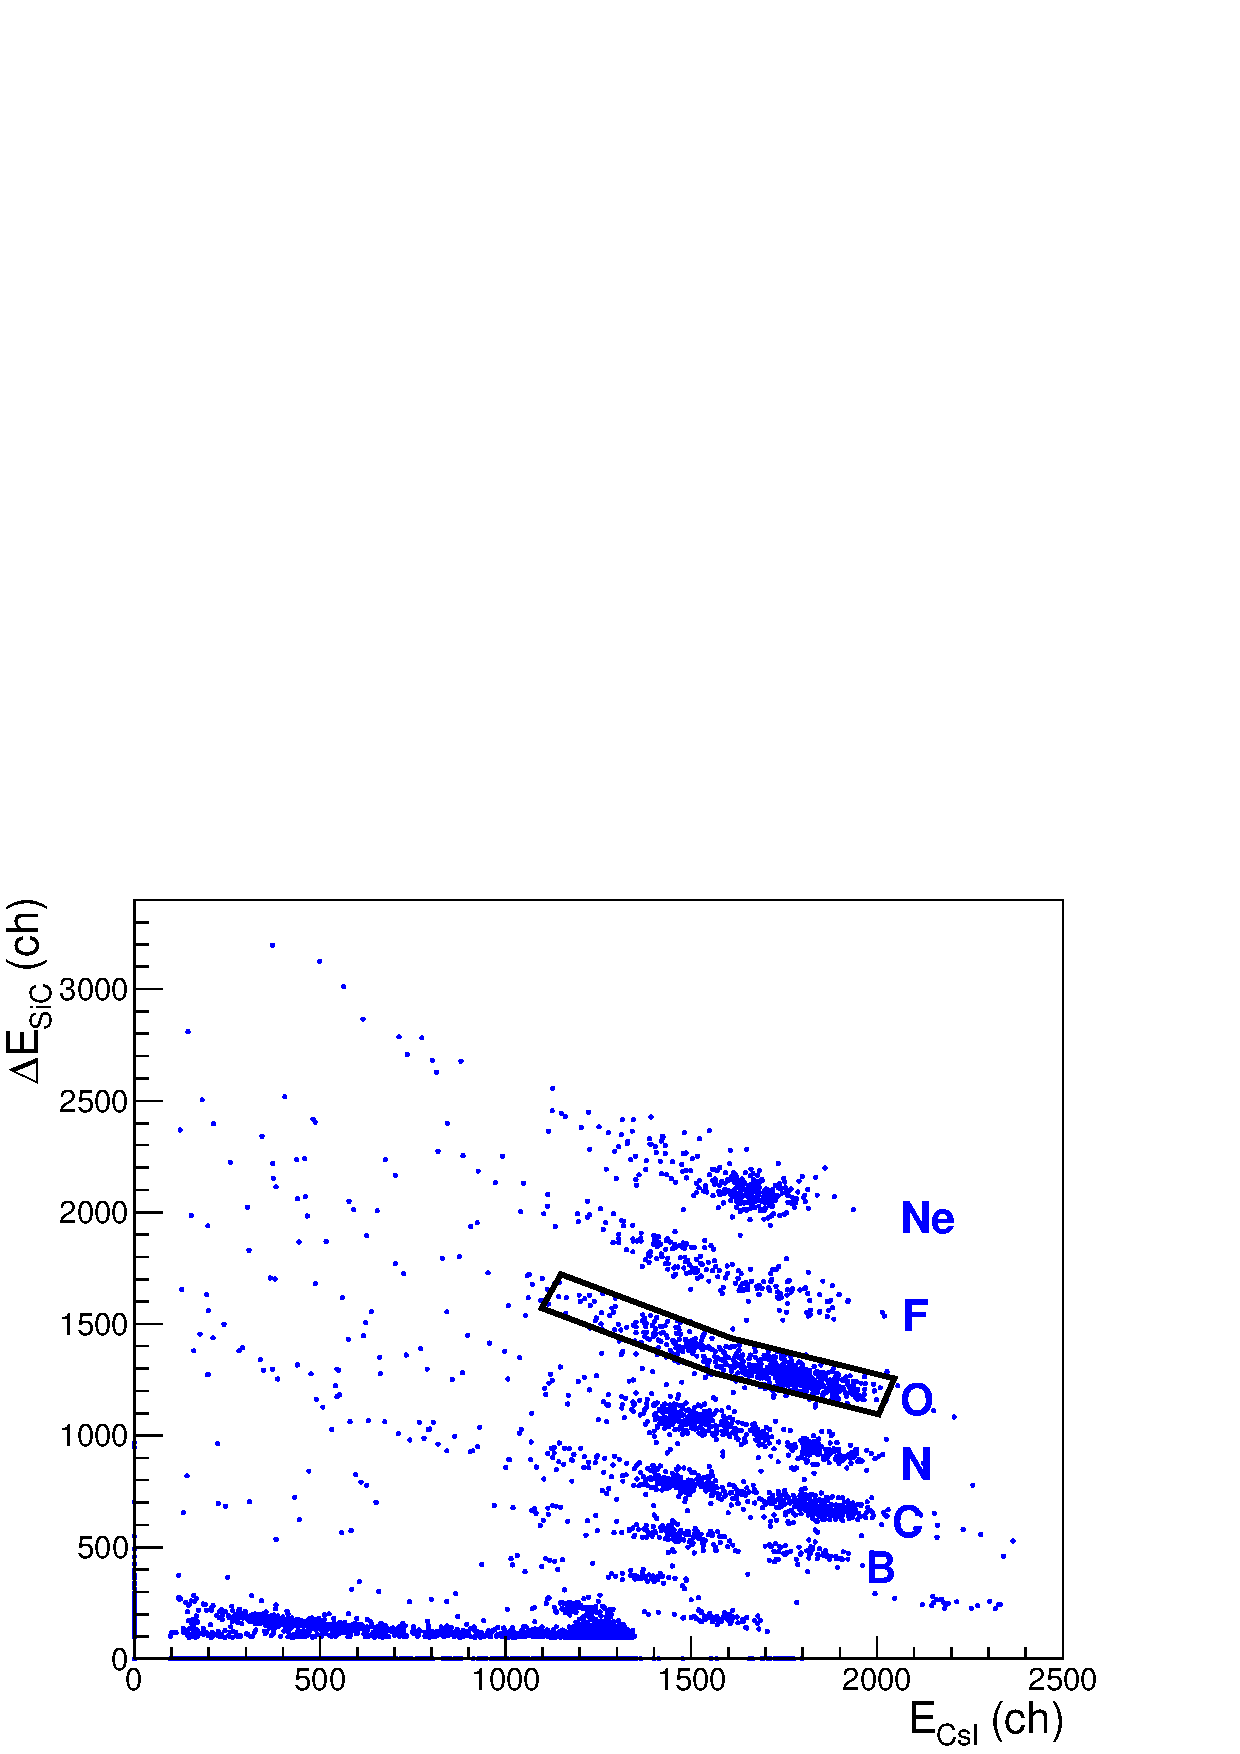
\includegraphics[width=\textwidth, keepaspectratio]{Grafici_Tesi/Test/matrice_sic_csi_taglio3.png}
	\caption{Le correlazioni $\Delta E_{SiC} - E_{CsI}$ ottenute dal Tel~A durante il test. La linea nera indica il taglio grafico effettuato per la selezione in numero atomico dell'Ossigeno.} \label{fig:sic_csi_standard}
\end{figure}

%Alla luce di questo risultato, il telescopio SiC-CsI sembra, dunque, rispondere alle richieste del progetto.
%Ricordando che questo telescopio era montato in configurazione reverse, si può anche osservare che il substrato epitassiale da 100~$\mu$m non sembra influire negativamente sulle sue proprietà di identificazione. 

%Ciò consente, dunque, di selezionare 

%Per confrontare le prestazioni di questo sistema con quelle solitamente ottenute utilizzando la co


%A questo punto può essere utile confrontare le prestazioni di questo sistema con quelle dell'apparato standard di MAGNEX, nel quale l'identificazione in numero atomico degli ioni avviene correlando la misura dell'energia persa $\Delta E$ nel gas con quella dell'energia residua $E_{resid}$ nei rivelatori al silicio; in particolare, la perdita di energia nel gas è data dalla somma delle sei perdite di energia $\Delta E_i$ misurate dai fili proporzionali.
%Inoltre, dal momento che la perdita di energia dipende dalla lunghezza della traiettoria dello ione all'interno del FPD, essa viene corretta, evento per evento, moltiplicando per il coseno dell'angolo di incidenza $\theta_{foc}$, ovvero 
%\begin{equation}
%	\Delta E^{corr}_{tot} \, = \, \frac{\cos \theta_{foc}}{\cos \theta_{tilt}} \, \sum_{i=1}^{6} \Delta E_i
%\end{equation}
%laddove $\theta_{tilt}$ rappresenta l'angolo di rotazione del FPD, pari a 59.2\textdegree.
In Figura~ si riporta la  matrice $\Delta E_{SiC} - E_{CsI}$ ottenuta con lo stesso telescopio utilizzando l'elettronica VMM3a: in questo caso si può notare che, sebbene si possano ancora riconoscere i luoghi corrispondenti ai diversi ioni, le curve sono parzialmente sovrapposte.
Ciò deriva da un maggiore contributo del rumore elettronico e da un peggiore accoppiamento fra i rivelatori e l'elettronica di front-end.
Dal momento che i dati relativi all'elettronica VMM3a non consentono un'agevole identificazione, si è scelto di analizzare soltanto quelli ottenuti utilizzando l'elettronica standard.



\section{\iflanguage{italian}{Analisi dei dati del test beam}{Analysis of test beam data}}

Per poter confrontare i dati sperimentali con i risultati delle simulazioni è necessario che queste riproducano nel modo più fedele possibile le condizioni sperimentali.
Dunque, è stata svolta un'analisi dei dati raccolti durante il test per estrarre delle informazioni da inserire opportunamente nella simulazione.
In primo luogo, è necessario stabilire quali ioni debbano costituire le particelle primarie nella simulazione, per cui è stata svolta un'identificazione dei prodotti di reazione.
%Inoltre, poiché l'energia delle particelle primarie è un parametro di fondamentale importanza, è stata determinare l'energia con cui gli ioni incidevano sul telescopio.
Inoltre, dal momento che un altro parametro di fondamentale importanza riguarda l'energia delle particelle, è stata condotta un'analisi per determinare l'energia di incidenza degli ioni sul telescopio.


%Ciò è stato possibile grazie alla correlazione tra posizione ed energia indotta dalla forza di Lorentz: 

\subsection{\iflanguage{italian}{Identificazione dell'\ce{^{16}O}}{Identification of \ce{^{16}O}}}

A causa della bassa statistica raccolta durante il test, è stato deciso di simulare soltanto la specie atomica più abbondante nel campione.
%, che, come si può evincere dalla Figura~, risulta essere l'Ossigeno.
La prima fase nella procedura di identificazione consiste nel determinare il numero atomico $Z$ delle particelle rivelate: tale informazione è stata ricavata dalle matrici $\Delta E_{SiC} - E_{CsI}$ in Figura~\ref{fig:sic_csi_standard}, dove si può notare che la specie atomica maggiormente presente è l'Ossigeno (O). 

Dopo avere selezionato gli ioni O è necessario distinguerne gli isotopi in numero di massa $A$; a tale scopo, si è sfruttata la correlazione tra posizione ed energia indotta dalla forza di Lorentz: ricordando la~\ref{eq:legge_spettrometri_approx}, è possibile notare che la correlazione $x_{foc} - E_{resid}$ permette di separare gli ioni in base al loro rapporto $\sqrt{m}/q$, laddove $m$ e $q$ rappresentano, rispettivamente, la massa e la carica della particella.
Nel caso del telescopio, la quantità $E_{resid}$ corrisponde con buona approssimazione a $E_{CsI}$.
La matrice $x_{foc} - E_{CsI}$ è mostrata in Figura~\ref{fig:xfoc2_csi_standard}, dove è possibile osservare che gli isotopi dell'O originati dall'interazione proiettile-bersaglio sono prevalentemente \ce{^{16}O}, \ce{^{17}O} e \ce{^{18}O}.
Si sottolinea che nella correlazione $x_{foc} - E_{resid}$ il numero di massa cresce spostandosi verso sinistra poiché, per mantenere lo stesso valore di $x_{foc}$, se la massa aumenta $E_{resid}$ deve diminuire.
Come si può notare dalla Figura~\ref{fig:xfoc2_csi_standard}, l'isotopo più abbondante dell'O presente nel campione è \ce{^{16}O}, la cui comparsa è probabilmente favorita poiché deriva da un processo di trasferimento di una particella $\alpha$ dal proiettile al bersaglio. 

\begin{figure} [!p]
	\centering
	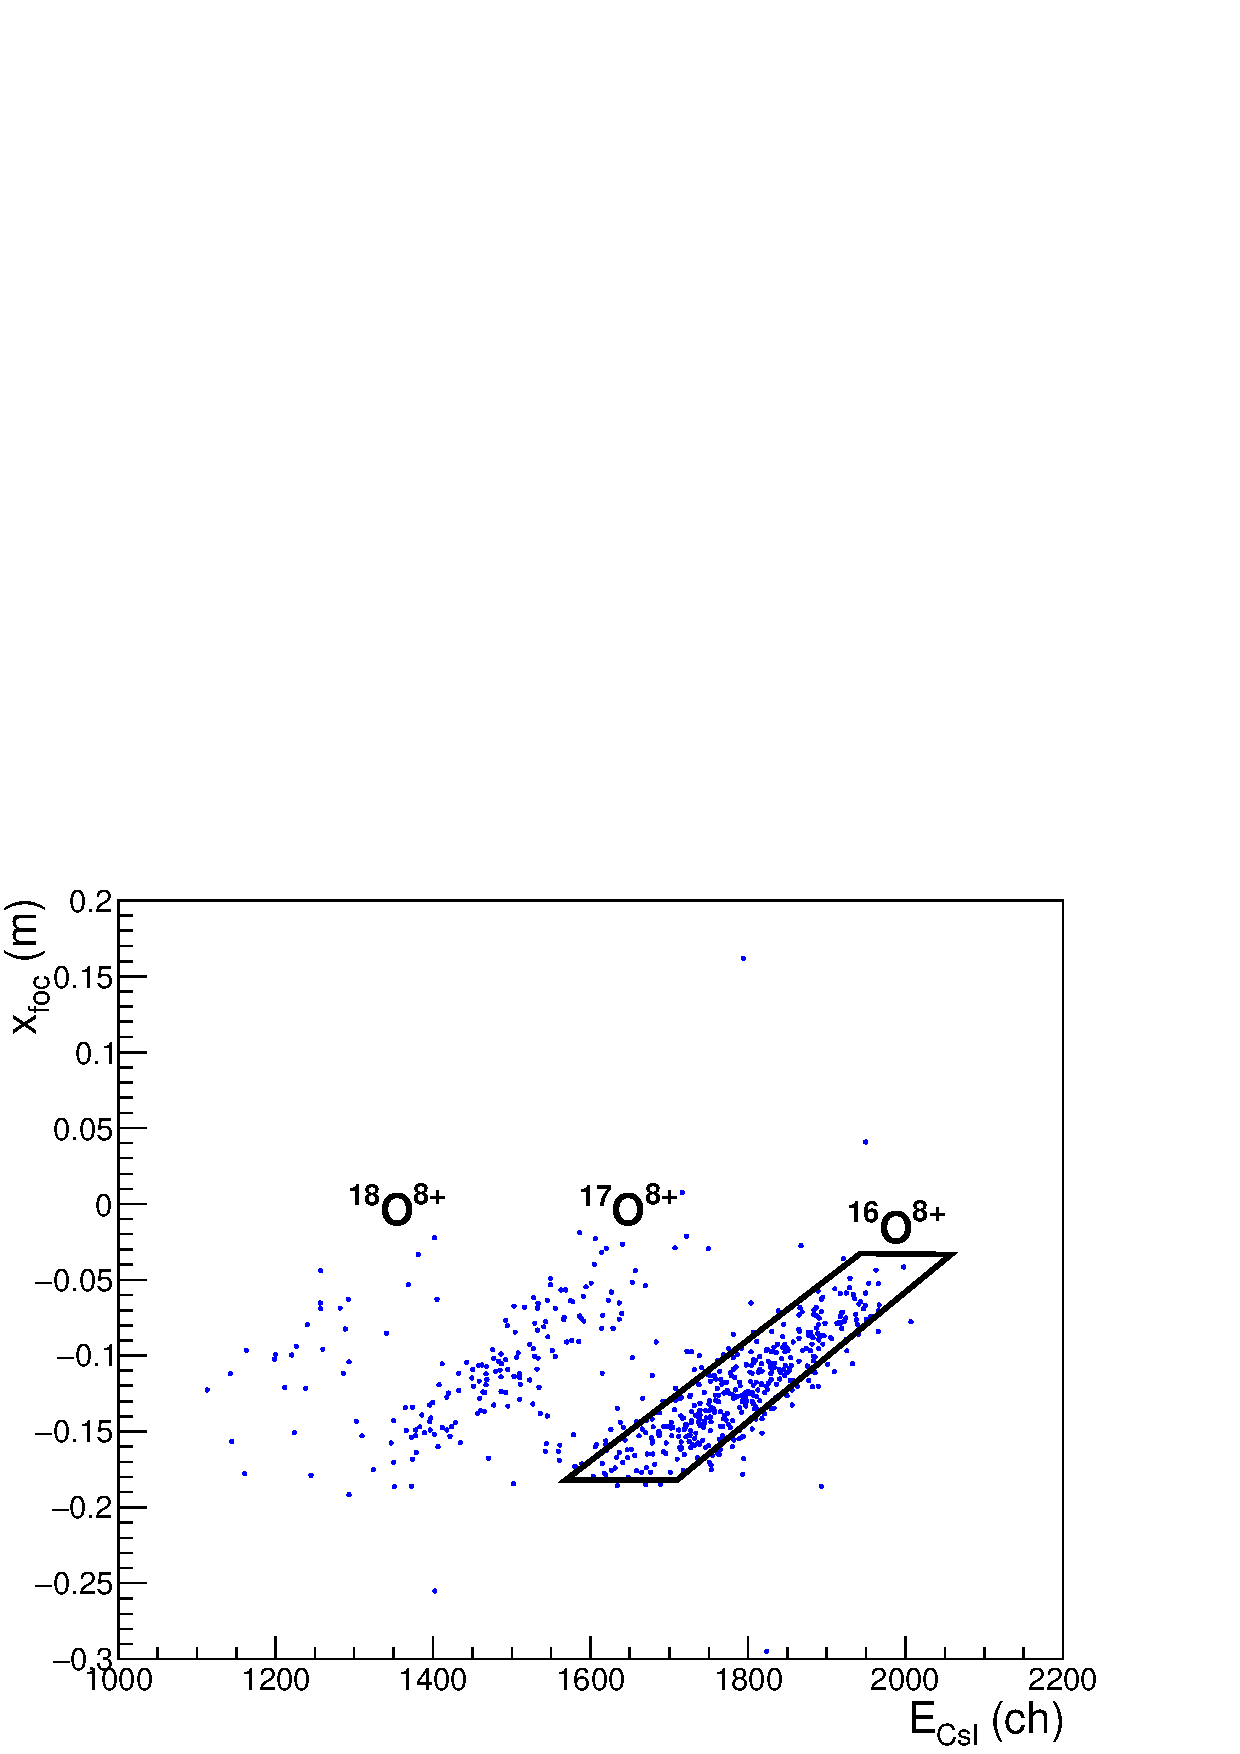
\includegraphics[width=\textwidth, keepaspectratio]{Grafici_Tesi/Test/matrice_xfoc2_csi_taglio.png}
	\caption{Le correlazioni $x_{foc} - E_{CsI}$ ottenute, durante il test, dalla misura in correlazione del tracciatore e del rivelatore allo CsI . La linea nera indica il taglio grafico effettuato per la selezione in numero atomico dell'\ce{^{16}O}.} \label{fig:xfoc2_csi_standard}
\end{figure}



\subsection{\iflanguage{italian}{Determinazione dell'energia dell'\ce{^{16}O}}{Energy determination of \ce{^{16}O}}}

Una volta identificato l'isotopo, è possibile determinare la sua energia cinetica $E_{kin}$ all'ingresso del rivelatore di piano focale (Focal Plane Detector, FPD) grazie alla correlazione tra l'angolo orizzontale $\theta_{foc}$ della traccia al piano focale e la coordinata orizzontale $x_{foc}$ del punto di arrivo della particella sullo stesso piano.
Ciascuno dei rivelatori di stop del FPD, indipendentemente dal fatto che si tratti di un rivelatore al silicio o di un telescopio, corrisponde ad una certa posizione $x_{foc}$; in particolare, dal momento che i rivelatori hanno superficie finita, ognuno di loro copre un'intervallo di posizioni in $x_{foc}$, legato alla propria estensione.
%Dunque, ricordando la~\ref{eq:legge_spettrometri_approx}, è possibile affermare che una misura di $x_{foc}$ equivale ad una misura dell'energia.
Dunque, ricordando la~\ref{eq:legge_spettrometri_approx}, è possibile affermare che, fissato lo ione, esso può arrivare in un certo intervallo in $x_{foc}$ soltanto con un determinato range energetico; in altre parole, gli ioni di \ce{^{16}O} che incidevano sul telescopio dovevano necessariamente avere degli specifici valori di energia.
Tali valori di energia sono correlati alle corrispondenti variabili $\theta_{foc}$ attraverso la cinematica della reazione $^{12}\mbox{C}\,  ( ^{20}\mbox{Ne}, ^{20}\mbox{O} ) \, ^{16}\mbox{O} $.

La matrice $\theta_{foc} - x_{foc}$ è riportata in Figura~\ref{fig:tefoc_xfoc2}, dove in rosso sono rappresentati i dati relativi al Tel~A, mentre in blu sono indicati i dati dello stesso ione, identificati tramite le tecniche di identificazione standard di MAGNEX.
\begin{figure} [!p]
	\centering
	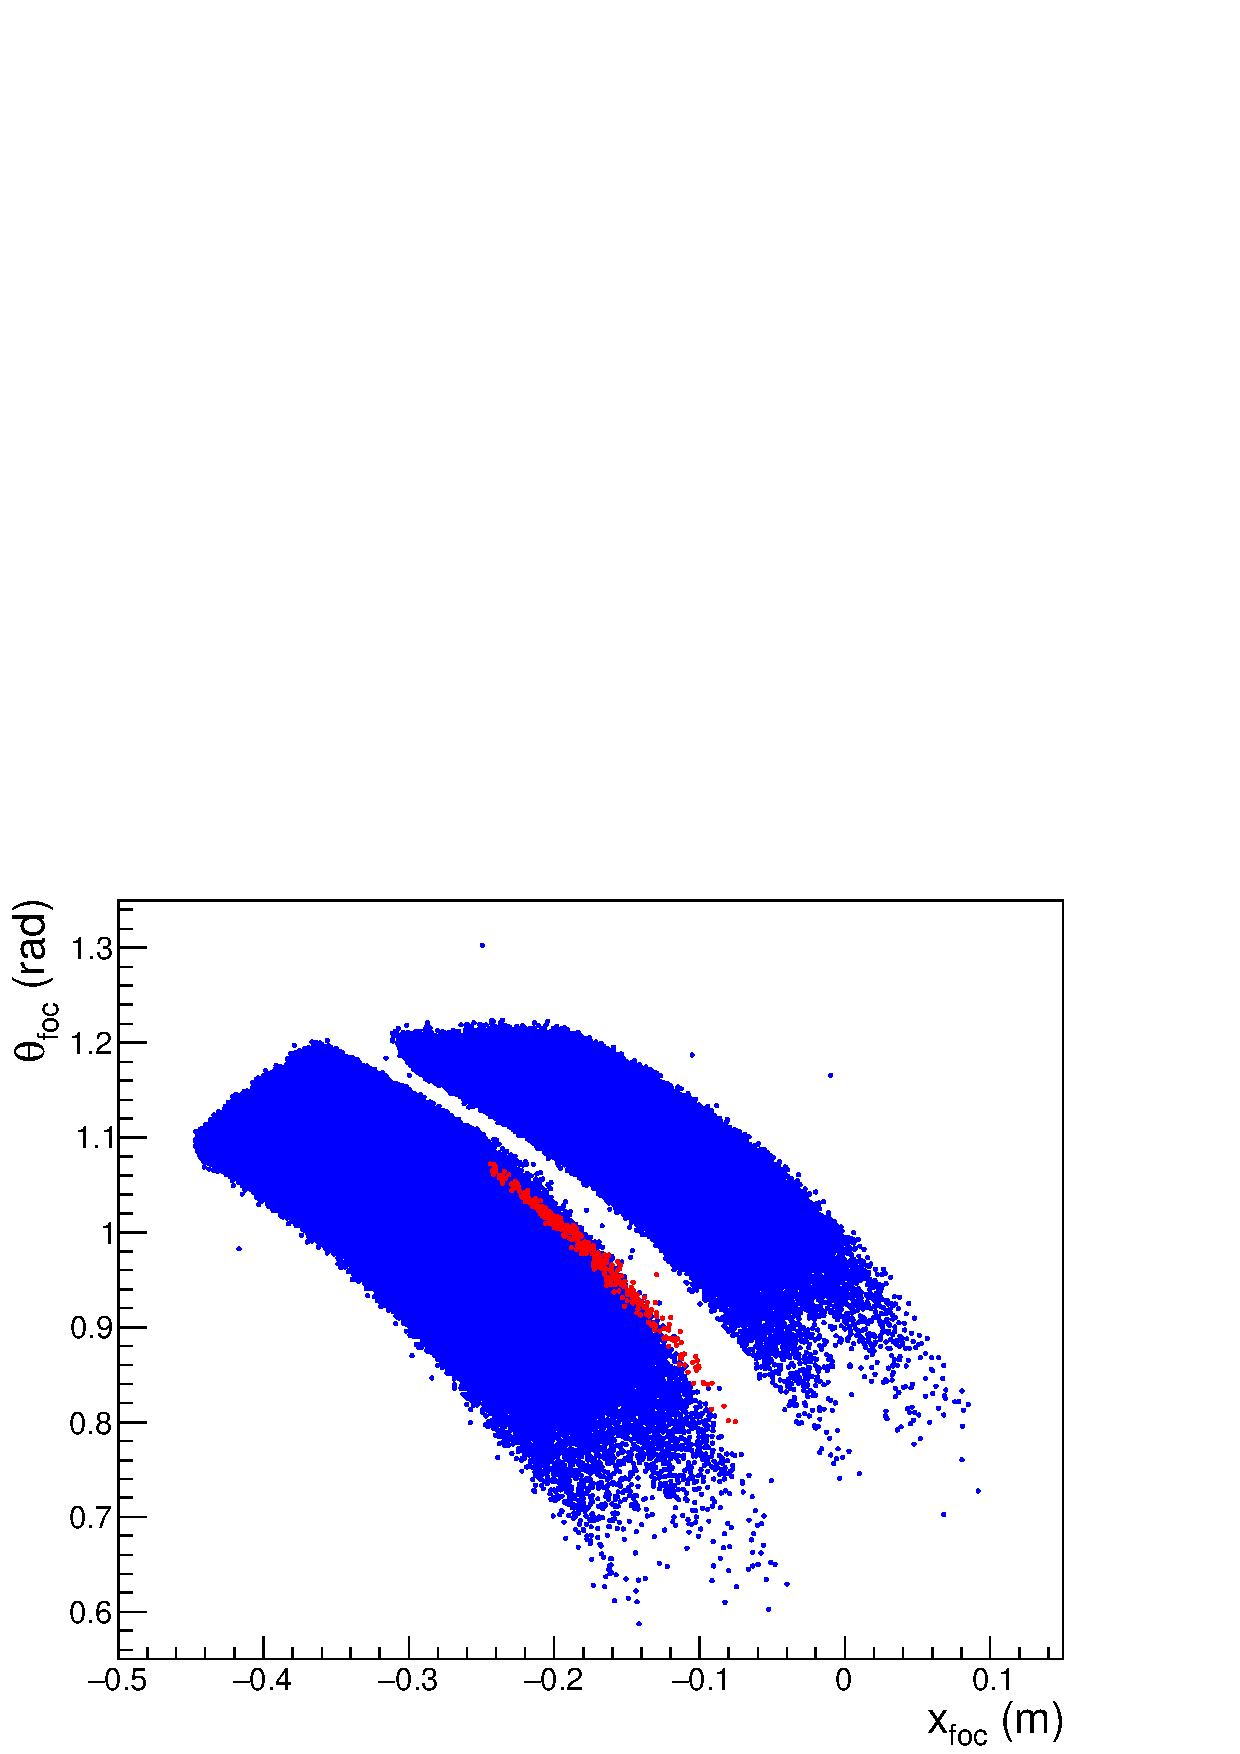
\includegraphics[width=\textwidth, keepaspectratio]{Grafici_Tesi/Test/matrice_tefoc_xfoc.png}
	\caption{Le correlazioni $\theta_{foc} - x_{foc}$ ottenute, durante il test, dalla misura in correlazione dell'angolo della traccia al piano focale e della posizione di arrivo allo stesso piano. Le matrici all'\ce{^{16}}: in blu sono riportati i dati misurati con i rivelatori standard di MAGNEX, in rosso sono mostrati i dati raccolti con il Tel~A.} \label{fig:tefoc_xfoc2}
\end{figure}
Come si può notare, la larghezza della striscia rossa è molto inferiore rispetto a quella delle strisce blu: ciò dipende dalla grande differenza fra la superficie del telescopio, pari a $1 \times 1$~cm\ap{2}, e quella dei rivelatori al silicio, ciascuna uguale a $5 \times 7$~cm\ap{2}.
In questo caso, le variabili $\theta_{foc}$ e $x_{foc}$ sono calibrate e sono misurate, rispettivamente, in radianti e metri.
Per determinare il range energetico all'interno del quale gli ioni di \ce{^{16}O} arrivavano sul telescopio, è sufficiente conoscere i valori di energia corrispondenti ai due estremi della striscia rossa.
Sebbene, in base a quanto detto, potrebbe sembrare possibile estrarre tale informazione a partire dalla sola misura della coordinata $x_{foc}$, in realtà, un punto della matrice $\theta_{foc} - x_{foc}$ potrebbe essere occupato da uno ione in uno stato eccitato.
È stata, quindi, svolta una simulazione, basata su metodi Monte Carlo, allo scopo di generare in modo casuale i parametri fisici dei prodotti della reazione in esame.
In tale simulazione sono stati presi in considerazione diversi stati eccitati dell'\ce{^{16}O} e, tramite una scelta accurata, si è fatto in modo che due di questi passassero per gli estremi della regione pertinente al telescopio.
Il risultato di tale procedura è mostrato in Figura~\ref{fig:simulazione}, dove, sovrapposti alle matrici precedentemente descritte, appaiono in nero i luoghi corrispondenti alle energie di eccitazione considerate.
\begin{figure} [!p]
	\centering
	\includegraphics[width=\textwidth, keepaspectratio]{Grafici_Tesi/Test/simulazione.png}
	\caption{Il risultato della simulazione della reazione $^{12}\mbox{C}\,  ( ^{20}\mbox{Ne}, ^{20}\mbox{O} ) \, ^{16}\mbox{O} $ per diverse energie di eccitazione dell'\ce{^{16}O}.} \label{fig:simulazione}
\end{figure}
Come si può notare, gli ioni di \ce{^{16}O} si trovano in uno stato altamente eccitato, laddove gli estremi della regione del telescopio sono attraversati dagli stati eccitati a 38 e 72~MeV, mentre gli altri due stati a 55 e 65~MeV si posizionano circa a metà di tale regione.
%Nota questa informazione, si è utilizzato il software di cinematica CATKIN, grazie al quale, introducendo gli opportuni valori di energia cinetica del proiettile e di energia di eccitazione del l'eiettile, si è ricavata la correlazione l'energia cinetica dell'eiettile ad un determinato angolo di emissione.
%Nota questa informazione, per calcolare l'energia cinetica dell'eiettile si è utilizzato il software di cinematica CATKIN, nel quale vengono tenuti in considerazione i parametri rilevanti come energia di eccitazione e angolo di emissione. 
La simulazione permette, inoltre, di conoscere, evento per evento, l'energia cinetica dell'eiettile, nonché l'angolo di emissione $\theta_{p}$.
È bene sottolineare che tale angolo non coincide con $\theta_{foc}$, ma esiste una relazione empirica fra le due quantità, ovvero
\begin{equation}
	\theta_{p} = \frac{\theta_{foc} - \theta_{tilt}}{-2.7} + \ang{10}
\end{equation}
dove $\theta_{tilt}$ denota l'angolo di rotazione del FPD, $-2.7$ rappresenta l'ingrandimento angolare di MAGNEX e 10\textdegree{} indica l'angolo ottico dello spettrometro.
Prendendo in considerazione i quattro stati simulati è stato possibile ricavare quattro coppie $(\theta_{foc} , E_{kin})$, sulle quali è stato effettuato un fit lineare allo scopo di derivare una relazione fra le due grandezze.
La retta trovata ha la seguente equazione:
\begin{equation} \label{eq:correlazione_angolo_energia}
	\theta_{foc} \, = \, -0.012 \, E_{kin} + 4.588
\end{equation}

Grazie alla~\ref{eq:correlazione_angolo_energia} è possibile trasformare una misura di angolo in una misura di energia.
Dunque, gli eventi relativi al Tel~A nella matrice $\theta_{foc} - x_{foc}$ sono stati proiettati sull'asse verticale, ottenendo lo spettro energetico riportato in Figura~, il quale riproduce la distribuzione in energia cinetica degli ioni di \ce{^{16}O} all'ingresso del FPD.
Tali energie non corrispondono a quelle di incidenza sul telescopio, in quanto i prodotti di reazione devono prima attraversare la finestra di Mylar e il tracciatore a gas.
Sono state, quindi, calcolate le perdite di energia in queste due componenti grazie al software LISE++, variando opportunamente l'energia cinetica e l'angolo della particella.
Alla fine di tale procedura è stato possibile stimare che il range di energia con cui gli ioni di \ce{^{16}O} giungevano sul Tel~A era compreso tra 290 e 310~MeV.



\section{\iflanguage{italian}{Confronto fra i dati del test e la simulazione \geant}{Comparison between test data and \geant simulation}}

Noti tutti i parametri rilevanti, è stata svolta una simulazione per cercare di riprodurre lo spettro sperimentale. 
Dal momento che il processo di produzione degli ioni di \ce{^{16}O} nell'interazione fra proiettile e bersaglio è governato da una sezione d'urto che varia in funzione dell'energia, era necessario introdurre nella simulazione una ``modulazione'' del numero di particelle primarie generate rispetto all'energia.
A tal fine, si è eseguito un fit con un polinomio del quarto ordine sullo spettro in Figura~, ottenendo il risultato riportato in Figura~.
La distribuzione dell'energia cinetica delle particelle primarie deve, dunque, rispecchiare l'andamento di tale funzione di fit.
Nella simulazione si è provato ad ``imitare'' la sezione d'urto della reazione definendo una variabile che svolgesse il ruolo di probabilità del processo.
Venivano, dunque, estratte in modo casuale ed uniforme l'energia della particella nel range compreso tra 290 e 310~MeV 



\cleardoublepage
\phantomsection
\chapter*{\iflanguage{italian}{Conclusioni}{Conclusions}}
\addcontentsline{toc}{chapter}{\iflanguage{italian}{Conclusioni}{Conclusions}}
\markboth{Conclusioni}{Conclusioni}

%Le simulazioni computerizzate costituiscono oggi un potente strumento per studiare la risposta di un sistema di rivelazione e per analizzarne il comportamento al variare delle sue caratteristiche.
%Le simulazioni numeriche costituiscono un potente strumento per studiare la risposta di un sistema di rivelazione e per ottimizzarne le caratteristiche tecniche.

Le simulazioni numeriche costituiscono nella fase di progettazione di un sistema di rivelazione un potente strumento per studiarne la risposta e per ottimizzarne le caratteristiche tecniche.
Per questo motivo, il progetto NUMEN, che ha avviato una radicale ristrutturazione dello spettrometro magnetico MAGNEX, ha deciso di dotarsi di una simulazione dell'apparato sperimentale previsto.
%Dal momento che il progetto NUMEN ha avviato una radicale ristrutturazione del proprio apparato sperimentale, 
%Nell'ambito del progetto NUMEN è stata realizzata una simulazione basata sulla piattaforma \geant{}, allo scopo di valutare le prestazioni di un sistema per la rivelazione e l'identificazione di ioni pesanti ad alto rate, costituito da un muro di telescopi $\Delta E - E_{resid}$ a stato solido.
In occasione di questo lavoro di tesi, è stato sviluppato e implementato, per la prima volta, un tool di simulazioni capace di descrivere in modo completo la cinematica di reazione, il moto degli eiettili attraverso lo spettrometro e l'interazione di questi con un muro di telescopi $\Delta E - E$ a stato solido.
%
%Tale tool si compone essenzialmente di due parti: la prima ricostruisce la traiettoria degli ioni nello spettrometro, la seconda simula l'interazione ione-rivelatore.
%A causa della grande accettanza in angolo solido e in impulso di MAGNEX, la ricostruzione della traiettoria degli ioni richiede il calcolo della matrice del trasporto fino al decimo ordine.
%Questa complessa operazione viene svolta all'interno del tool da software sviluppati all'uopo e ottimizzati dalla collaborazione NUMEN.
%Essi sono basati sugli algoritmi di COSY INFINITY 
Tale tool si compone essenzialmente di due parti: la prima, dedicata alla ricostruzione della traiettoria degli ioni nello spettrometro, è costituita da software sviluppati all'uopo e ottimizzati dalla collaborazione NUMEN, la seconda, che simula l'interazione ione-rivelatore, è basata su un'applicazione \geant.
%Il motivo alla base di questa strutturazione del tool deriva dal fatto che, a causa della grande accettanza in angolo solido e in impulso di MAGNEX, la ricostruzione della traiettoria degli eiettili richiede la risoluzione delle equazioni del moto fino al decimo ordine e, pertanto, necessita di software specifici.
L'integrazione tra le due parti e la realizzazione di tale applicazione sono state gli obiettivi principali di questo lavoro di tesi.
All'interno del progetto NUMEN, il tool assume una notevole importanza, perché, in primo luogo, aiuta a progettare l'apparato sperimentale, suggerendo le condizioni ottimali in merito alla geometria e alle specifiche dei rivelatori. 
Inoltre, esso ottimizza la spesa economica e di man-power, riducendo i costi di produzione e gestione del progetto.

In questo lavoro, il tool è stato utilizzato per valutare le capacità di Particle IDentification (PID) di un sistema di telescopi basato sulla tecnologia SiC-CsI; in particolare, il primo sistema preso in considerazione era costituito da dispositivi con dimensioni trasversali di 1.5~cm $\times$ 1.5~cm.
Tale sistema si è dimostrato in grado di separare efficacemente gli ioni sia in numero atomico sia in numero di massa.
Si è, tuttavia, osservato che la presenza, attorno alla parte sensibile del rivelatore al~SiC, di una cornice in cui la carica prodotta dal passaggio degli ioni viene parzialmente raccolta genera degli eventi degradati, i quali costituiscono un fondo nella PID, poiché possono disporsi sul luogo caratteristico di uno ione diverso.
Inoltre, una seconda sorgente di fondo è rappresentata dagli ioni che, a causa dell'inclinazione della loro traiettoria, non si fermano nel cristallo di~CsI e rilasciano, dunque, solo una parte della loro energia residua.
%Tale tool è strutturato in modo che 
%Per poter riprodurre il comportamento reale degli ioni nello spettrometro, il tool è stato realizzato incorporando le correlazioni dovute sia alla cinematica sia alle proprietà ottiche dello spettrometro.
%Poiché tali correlazioni sono caratterizzate da effetti non-lineari e richiedono la risoluzione di complesse equazioni, si è scelto  
%Tale tool integra i software per il calcolo della cinematica e della matrice del trasporto degli eiettili attraverso MAGNEX con un'applicazione specifica basata sulla piattaforma \geant.
%Dal momento che la cinematica e le proprietà ottiche dello spettrometro introducono delle correlazioni non-lineari che difficil
%Dal momento che tale sistema verrà utilizzato per rivelare i prodotti di reazione deg
%Tale simulazione ha permesso di verificare che una soluzione basata sulla tecnologia SiC-CsI può soddisfare le performance necessarie per gli obiettivi del progetto, garantendo una buona separazione degli ioni di interesse per NUMEN lungo tutto il range energetico preso in considerazione.
%Dal momento che il progetto intende studiare le reazioni di doppio scambio di carica (Double Charge Exchange, DCE), le quali sono caratterizzate da sezioni d'urto estremamente basse, un importante aspetto di questo lavoro è consistito nello stimare la percentuale di contaminazioni nella regione di interesse (Region Of Interest): in tutti i casi esaminati, tale quantità è risultata inferiore ai limiti imposti sulla perdita di segnali corretti e sulla contaminazione originata dal fondo.
Dal momento che il progetto intende studiare le reazioni di doppio scambio di carica (Double Charge Exchange, DCE), le quali sono caratterizzate da sezioni d'urto estremamente basse (tipicamente di poche decine di~nb), la percentuale di eventi di fondo nella regione di interesse (Region Of Interest, ROI) deve essere piccola rispetto al segnale.
Un importante aspetto di questo lavoro è, dunque, consistito nella valutazione della percentuale di contaminazione e nel calcolo del rapporto segnale-background (S/B) nella ROI. 
I valori delle contaminazioni determinati con le simulazioni sono stati opportunamente riscalati per le sezioni d'urto di produzione dei diversi ioni, in modo da ottenere delle stime realistiche.
Dal calcolo è emerso che, nello studio di una reazione di DCE a bassa energia di eccitazione, il principale contaminante allo ione di interesse (\ce{^{20}O}) è il \ce{^{20}F^{8+}}, il quale è originato da un processo di singolo scambio di carica (Single Charge Exchange, SCE). 
Tuttavia, alle energie di fascio considerate, la probabilità di ottenere lo stato di carica $8+$ per uno ione di \ce{^{20}F} è molto piccola; infatti, calcolando il rapporto S/B, è stato possibile dimostrare che la sensibilità di misura dell'apparato simulato nella ROI è di 200~pb a 5$\sigma$, quindi ben sufficiente a misurare la reazione di interesse.


È stato, inoltre, osservato che, ai fini della PID, la correlazione $\Delta E_{SiC} - E_{CsI}$ produce prestazioni non lontane da quelle della correlazione $\Delta E_{SiC} - E_{meas}$, laddove $\Delta E_{SiC}$ indica la perdita di energia nel rivelatore al~SiC, $E_{CsI}$ l'energia residua rilasciata nel cristallo allo~CsI ed $E_{meas}$ la somma delle due precedenti.
In particolare, nel caso di telescopi da 1.5~cm $\times$ 1.5~cm, è stata stimata una sensibilità di misura di 460~pb a 5$\sigma$.
Questo risultato ha permesso di concludere che per l'identificazione degli ioni non è necessario sommare le energie misurate dai due stadi del telescopio, rendendo, dunque, non necessaria la calibrazione dei rivelatori.
%rendendo, dunque, non necessaria la calibrazione dei due stadi del telescopio.

Le capacità di PID del telescopio sono state valutate anche nello studio di una reazione di DCE ad elevata energia di eccitazione.
In questo caso, i maggiori contaminanti sono originati dai processi di 1-neutron e 1-proton stripping (rispettivamente \ce{^{19}Ne^{10+}} e \ce{^{19}F^{9+}}) e dal SCE (\ce{^{20}F^{9+}}).
A causa della grande probabilità di ottenere questi ioni in questi stati di carica, le percentuali di contaminazione riscontrate sono elevate; infatti, la sensibilità di misura è risultata essere di 300~$\mu$b a 5$\sigma$, estremamente più grande di quella necessaria per osservare il DCE.
Tuttavia, è stato dimostrato che la misura del tempo di volo degli ioni potrebbe permettere di separare lo ione di interesse da tali contaminanti, purché la risoluzione su tale quantità sia inferiore ai 10~ns.
Pertanto, la sensibilità di misura complessiva dell'apparato potrebbe essere, anche in questo caso, sufficiente per osservare il DCE.


%Diversi studi sono stati condotti variando le dimensioni trasversali dei rivelatori, dai quali è emerso che la percentuale di eventi affetti da raccolta di carica incompleta, principale fonte di errore nell'identificazione, diminuisce all'aumentare della superficie sensibile.
Un aspetto rilevante di questo lavoro è consistito nell'ottimizzazione della granularità dei telescopi: oltre al caso di 1.5~cm $\times$ 1.5~cm, sono stati presi in considerazione dispositivi da 1~cm $\times$ 1~cm e da 2~cm $\times$ 2~cm.
In questo studio si è verificato che, all'aumentare della superficie di rivelazione, la sensibilità di misura diminuisce; essa resta, però, anche in questi due casi sufficiente per misurare il DCE.
In condizioni di alti flussi di particelle incidenti, come quelli previsti per NUMEN, un fenomeno da tenere in considerazione per la scelta delle dimensioni dei rivelatori è il pile-up.
È stato, dunque, effettuato un calcolo analitico allo scopo di studiare l'andamento della probabilità di pile-up al variare della superficie del rivelatore, dal quale è risultato che tale quantità aumenta velocemente al crescere delle dimensioni trasversali.
Inoltre, sulla scelta della granularità da adottare entrano in gioco anche altri fattori, legati, ad esempio, al numero totale di dispositivi e al numero di canali necessari per leggere tali dispositivi.
%Di conseguenza, dal compromesso tra le due esigenze, si è dedotto che la configurazione ottimale per gli scopi del progetto prevede l'utilizzo di telescopi da $1.5 \times 1.5$~cm\ap{2}.
Di conseguenza, bisogna cercare una soluzione di compromesso tra tutte le esigenze; da questo lavoro si può dedurre che tale soluzione è rappresentata dai telescopi da 1.5~cm $\times$ 1.5~cm.

%L'analisi dell'influenza degli effetti di bordo del rivelatore al SiC sulle capacità di PID ha consentito di sostenere che la percentuale di eventi degradati cresce all'aumentare della lunghezza della regione di transizione, ma resta comunque entro i limiti fissati.
%Dunque, anche nel caso in cui tali rivelatori dovessero avere una regione parzialmente attiva con una lunghezza maggiore dei 50~$\mu$m assunti come valore di riferimento, le prestazioni di identificazione non dovrebbero subire sostanziali peggioramenti.



%Lo studio sul substrato epitassiale del rivelatore al SiC ha fatto emergere che la riduzione dello spessore dai 350 ai 10~$\mu$m provoca un aumento della percentuale di eventi degradati, risultando in un peggioramento delle performance di PID.
%Dunque, dal punto di vista dell'identificazione, l'ablazione LASER del substrato si configura come un'operazione ingiustificata, nonché potenzialmente dannosa in termini di resa di produzione dei dispositivi.


%Un aspetto fondamentale di questo lavoro è consistito nella validazione della simulazione Monte Carlo attraverso il confronto con i dati sperimentali raccolti in occasione del test beam svolto ad Aprile 2019.
Un aspetto fondamentale di questo lavoro è consistito nella partecipazione al test beam svolto ad Aprile 2019, in occasione del quale si è contribuito all'assemblaggio dell'apparato sperimentale e alla fase di acquisizione dei dati.
%I dati sperimentali raccolti durante tale test sono stati messi a confronto 
Tale test aveva lo scopo di studiare le prestazioni del primo prototipo di telescopio SiC-CsI per NUMEN, utilizzando sia l'elettronica tradizionale di MAGNEX sia il primo esemplare di elettronica di front-end VMM3a realizzato per il progetto.
%I dati sperimentali sono stati analizzati allo scopo di ricostruire i parametri essenziali da introdurre nella simulazione, come ad esempio il numero atomico e il numero di massa della particella primaria e il range energetico.
I dati sperimentali raccolti in tale occasione sono stati utilizzati in questo lavoro per effettuare un confronto con i dati ottenuti dalla simulazione; per questo motivo, è stata svolta un'analisi su tali dati.
È stata, pertanto, eseguita un'identificazione degli eiettili utilizzando le correlazioni $\Delta E_{SiC} -E_{CsI}$ e $x_{foc} -E_{CsI}$, allo scopo di selezionare lo ione più abbondante nel campione, risultato essere l'\ce{^{16}O}.
%Grazie alla tecnica basata sulla deflessione causata dalla forza di Lorentz, è stato possibile ricavare la distribuzione in energia cinetica di tale ione, la quale è stata riprodotta all'interno della simulazione.
Noti l'eiettile da simulare, la tipologia e l'energia del fascio, è stato utilizzato il tool per verificare se i dati sperimentali venissero riprodotti correttamente.
Gli spettri energetici registrati dal rivelatore al SiC e dallo scintillatore allo CsI sono stati messi a confronti con i rispettivi spettri simulati: in entrambi i casi la compatibilità è significativa, in particolar modo per quanto riguarda il rivelatore al SiC.
Alla luce di questo accordo è possibile affermare che la simulazione riesce a riprodurre bene la realtà sperimentale, convalidando i risultati ottenuti nel corso di questo lavoro.





%Dal momento che, per raggiungere i propri obiettivi, il progetto deve spingersi al limite delle attuali possibilità nel campo degli esperimenti con fasci di ioni pesanti ad elevata intensità, è essenziale la ricerca e sviluppo di tecnologie di frontiera.
%In tale prospettiva si inquadra 
%Le stringenti esigenze di resistenza alle radiazioni hanno guidato verso la scelta di un primo stadio 
%%L'introduzione di tale sistema rientra in un più grande scenario che prevede una profonda opera di ristrutturazione del Ciclotrone Superconduttore K800 e dello spettrometro magnetico MAGNEX.
%Lo scopo di tale upgrade consiste nell'aum
%alla fine della quale sarà possibile ottenere fasci di ioni pesanti ad elevata intensità.
%%Tale upgrade ha l'obiettivo di aumentare l'intensità dei fasci di ioni pesanti attualmente disponibili di almeno due ordini di grandezza, al fine di poter avviare una campagna di studi sistematica di tutti gli isotopi coinvolti nel doppio decadimento beta senza neutrini (\doppiobeta).
%Tale condizione richiede un'intensa attività di ricerca e sviluppo in diversi campi della tecnologia coinvolta negli esperimenti 
%%Il raggiungimento di intensità così elevate rende necessaria un'intensa attività di ricerca e sviluppo in diversi campi della tecnologia coinvolta negli esperimenti di collisione di ioni pesanti; in particolare, innumerevoli studi sono stati dedicati all'analisi delle proprietà di resistenza alle radiazioni dei materiali e dei sistemi da utilizzare.
%in particolare, dal momento che la resistenza alle radiazioni è un requisito imprescindibile per la scelta dei materiali e dei sistemi da utilizzare, innumerevoli studi sono stati condotti 
%%Dal momento che i rivelatori al silicio non sono in grado di tollerare le intensità previste, il primo stadio del telescopio sarà basato su un rivelatore sottile (100~$\mu$m) al carburo di silicio (SiC), materiale che, grazie alle sue caratteristiche, ha attirato notevole interesse da parte della comunità scientifica.
%%Il rivelatore di stop del telescopio sarà, invece, costituito da un cristallo allo ioduro di cesio (CsI) dello spessore di 1~cm.
%Un'importante linea di ricerca è stata, dunque, avviata sulla realizzazione e caratterizzazione di rivelatori sottili basati su tale materiale.
%%Tuttavia, la resistenza alle radiazioni non è l'unico requisito che il sistema di identificazione deve possedere; infatti, esso deve in primo luogo consentire di discriminare in modo efficace gli ioni nella regione di interesse per NUMEN, costituita principalmente da Ossigeno, Fluoro e Neon.
%%Inoltre, esso deve possedere una risoluzione energetica tale da preservare le prestazioni dell'attuale apparato riguardo all'identificazione in numero atomico e numero di massa dei prodotti di reazione.










%\lipsum[20]


\cleardoublepage
\phantomsection
\addcontentsline{toc}{chapter}{\iflanguage{italian}{Bibliografia}{Bibliography}}
\bibliographystyle{mprsty}
\bibliography{biblio}


%\cleardoublepage
%\phantomsection
%\chapter*{\iflanguage{italian}{Ringraziamenti}{Acknowledgements}}
%\addcontentsline{toc}{chapter}{\iflanguage{italian}{Ringraziamenti}{Acknowledgements}}

%\lipsum[20]

\end{document}




